\documentclass[12pt]{elsarticle}
\usepackage[utf8]{inputenc}
%\usepackage{authblk}
\usepackage{setspace}
\usepackage[margin=0.75in]{geometry}
\usepackage{graphicx}
\graphicspath{ {./figures/} }
\usepackage[labelfont=bf, font = normalsize]{caption}
\usepackage{subcaption}
\usepackage{amsmath,amssymb,mathtools}
\usepackage{mathrsfs}
\usepackage{bm}
\usepackage{xcolor}
\usepackage{array}
\usepackage{appendix}
\usepackage{tikz}
\usepackage{floatrow}
\usepackage{rotating}
\usepackage{multirow,bigdelim}
\usepackage{array, blkarray, makecell}
\usepackage{tabularx}
\DeclareFloatFont{small}{\footnotesize}% "scriptsize" is defined by floatrow, "tiny" not
\floatsetup[table]{font=small}
\newcolumntype{P}[1]{>{\centering\arraybackslash}p{#1}}
\newcommand{\myparagraph}[1]{\paragraph{#1}\mbox{}\\}
\newcommand*\circled[1]{\tikz[baseline=(char.base)]{
            \node[shape=circle,draw,inner sep=2pt] (char) {#1};}}
\providecommand{\keywords}[1]
{
  \small	
  \textbf{\textit{Keywords:}} #1
}

\usepackage{siunitx}
\sisetup{per-mode = symbol}
\usepackage{tikz-3dplot}
\usepackage{graphicx}
\usetikzlibrary{calc,backgrounds}
\usepackage{pgfplotstable}
\usepgfplotslibrary{groupplots}
\usetikzlibrary{intersections}
\usetikzlibrary{positioning}
\usepgfplotslibrary{fillbetween}

%-Define RWTH colors----------------------------------------------------
\definecolor{rwth1}{RGB}{0,84,159}      % RWTH-Blau
\definecolor{rwth2}{RGB}{142,186,229}   % RWTH-Hellblau
\definecolor{rwth3}{RGB}{0,97,101}      % Petrol 
\definecolor{rwth4}{RGB}{0,152,161}     % Türkis
\definecolor{rwth5}{RGB}{87,171,39}     % Grün
\definecolor{rwth6}{RGB}{189,205,0}     % Maigrün
\definecolor{rwth7}{RGB}{255,237,0}     % Gelb
\definecolor{rwth8}{RGB}{246,168,0}     % Orange
\definecolor{rwth9}{RGB}{227,0,102}     % Magenta
\definecolor{rwth10}{RGB}{204,7,30}     % Rot
\definecolor{rwth11}{RGB}{161,16,53}    % Bordeaux
\definecolor{rwth12}{RGB}{97,33,88}     % Violett
\definecolor{rwth13}{RGB}{122,111,172}  % Lila

\definecolor{rwthb1}{HTML}{e8f1fa}      % RWTH-Blau1
\definecolor{rwthb2}{HTML}{c7ddf2}      % RWTH-Blau2
\definecolor{rwthb3}{HTML}{8ebae5}      % RWTH-Blau3
\definecolor{rwthb4}{HTML}{407fb7}      % RWTH-Blau4
\definecolor{rwthb5}{HTML}{00549f}      % RWTH-Blau5

\definecolor{rwtho1}{HTML}{fff7ea}      % RWTH-Orange1
\definecolor{rwtho2}{HTML}{feeac9}      % RWTH-Orange2
\definecolor{rwtho3}{HTML}{fdd48f}      % RWTH-Orange3
\definecolor{rwtho4}{HTML}{fabe50}      % RWTH-Orange4
\definecolor{rwtho5}{HTML}{f6a800}      % RWTH-Orange5

\definecolor{lightblue}{RGB}{173,216,230}

%-Define dash patterns--------------------------------------------------
\tikzstyle{dashpattern0} = [dash pattern = ]
\tikzstyle{dashpattern1} = [dash pattern = on 4.25pt off 0.75pt]
\tikzstyle{dashpattern2} = [dash pattern = on 1.5pt off 0.5pt]
\tikzstyle{dashpattern3} = [dash pattern = on 0.75pt off 0.4pt]
\tikzstyle{dashpattern4} = [dash pattern = on 3pt off 1pt on 1pt off 1pt]
\tikzstyle{dashpattern5} = [dash pattern = on 3.75pt off 0.5pt on 0.75pt off 0.5pt on 0.75pt off 0.5pt]
\tikzstyle{dashpattern6} = [dash pattern = on 3.25pt off 0.5pt on 0.75pt off 0.5pt on 0.75pt off 0.5pt on 0.75pt off 0.5pt]
\tikzstyle{dashpattern7} = [dash pattern = on 3.25pt off 0.5pt on 0.75pt off 0.5pt on 0.75pt off 0.5pt on 0.75pt off 0.5pt on 0.75pt off 0.5pt]
\tikzstyle{dashpattern8} = [line cap=round, dash pattern = on 3.25pt off 2.75pt]
\tikzstyle{dashpattern9} = [line cap=round, dash pattern = on 0.01pt off 2pt]
\tikzstyle{dashpattern10}= [line cap=round, dash pattern = on 3.25pt off 2pt on 0.01pt off 2pt]
\tikzstyle{dashpattern11}= [line cap=round, dash pattern = on 3.5pt off 1.75pt on 0.01pt off 1.75pt on 0.01pt off 1.75pt]
\tikzstyle{dashpattern12}= [line cap=round, dash pattern = on 3.5pt off 1.75pt on 0.01pt off 1.75pt on 0.01pt off 1.75pt on 0.01pt off 1.75pt]
\tikzstyle{dashpattern13}= [line cap=round, dash pattern = on 3.5pt off 1.75pt on 0.01pt off 1.75pt on 0.01pt off 1.75pt on 0.01pt off 1.75pt on 0.01pt off 1.75pt]

%-new commands
\newcommand{\tikzvdots}{%
  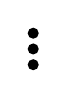
\begin{tikzpicture}[baseline=(current bounding box.center)]
    \fill (0,0) circle (2.0pt);
    \fill (0,-0.2) circle (2.0pt);
    \fill (0,-0.4) circle (2.0pt);
  \end{tikzpicture}%
}
\newcommand{\tightI}{\text{I}}
\newcommand{\tightII}{\text{I\hspace{-0.2mm}I}}
\newcommand{\tightIII}{\text{I\hspace{-0.2mm}I\hspace{-0.2mm}I}}
\newcommand{\tightIV}{\text{I\hspace{-0.2mm}V}}
            
\usepackage{tablefootnote}    
\usepackage{algorithm}
\usepackage{algpseudocode}

\usepackage{hyperref}

\usepackage{placeins}

\usepackage{amsthm}

% Define a new theorem-like environment for remarks
\newtheorem{remark}{Remark}  
            
%%%%%% Bibliography %%%%%%
% Replace "sample" in the \addbibresource line below with the name of your .bib file.

%\setcitestyle{authoryear,open={(},close={)}}
%\usepackage[style=ieee, 
%sorting=none]{biblatex}
%\setcitestyle{authoryear, open={[}, close={]}}
%\addbibresource{isrpaper.bib}

%%%%%% Title %%%%%%
% Full titles can be a maximum of 200 characters, including spaces. 
% Title Format: Use title case, capitalizing the first letter of each word, except for certain small words, such as articles and short prepositions
\usepackage{natbib}
\bibliographystyle{unsrtnat}
\title{%
	\Large A generalized dual potential for inelastic Constitutive Artificial Neural Networks: \large A JAX implementation at finite strains}

%%%%%% Authors %%%%%%
% Authors should be listed in order of contribution to the paper, by first name, then middle initial (if any), followed by last name.
% Authors should be listed in the order in which they will appear in the published version if the manuscript is accepted. 
% Use an asterisk (*) to identify the corresponding author, and be sure to include that person’s e-mail address. Use symbols (in this order: †, ‡, §, ||, ¶, #, ††, ‡‡, etc.) for author notes, such as present addresses, “These authors contributed equally to this work” notations, and similar information.

\author[1]{Hagen Holthusen \corref{cor1}}
\ead{hagen.holthusen@ifam.rwth-aachen.de}
\cortext[cor1]{Corresponding author\\hagen.holthusen@ifam.rwth-aachen.de\\ Mies-van-der-Rohe-Str. 1, 52074 Aachen, Germany}
\author[1,2]{Kevin Linka}
\author[3]{Ellen Kuhl}
\author[1]{Tim Brepols}

%%%%%% Affiliations %%%%%%
\address[1]{Institute of Applied Mechanics, RWTH Aachen University, Germany}
\address[2]{Institute for Continuum and Material Mechanics, Hamburg University of Technology, Germany}
\address[3]{Department of Mechanical Engineering, Stanford University, United States}
%\affiliation[*]{Corresponding author. Email: manjunatha@ifam.rwth-aachen.de}

%%%%%% Date %%%%%%
% Date is optional
\date{}

%%%%%% Spacing %%%%%%
% Use paragraph spacing of 1.5 or 2 (for double spacing, use command \doublespacing)
\onehalfspacing

\begin{document}

%%%%%% Abstract %%%%%%

\begin{abstract}
\begin{abstract}  
Test time scaling is currently one of the most active research areas that shows promise after training time scaling has reached its limits.
Deep-thinking (DT) models are a class of recurrent models that can perform easy-to-hard generalization by assigning more compute to harder test samples.
However, due to their inability to determine the complexity of a test sample, DT models have to use a large amount of computation for both easy and hard test samples.
Excessive test time computation is wasteful and can cause the ``overthinking'' problem where more test time computation leads to worse results.
In this paper, we introduce a test time training method for determining the optimal amount of computation needed for each sample during test time.
We also propose Conv-LiGRU, a novel recurrent architecture for efficient and robust visual reasoning. 
Extensive experiments demonstrate that Conv-LiGRU is more stable than DT, effectively mitigates the ``overthinking'' phenomenon, and achieves superior accuracy.
\end{abstract}  \\
\keywords{dual potential; neural network; finite strains; generalized standard materials; inelasticity; automated model discovery} 
\end{abstract}

\maketitle

\section{Introduction}
\label{sec:introduction}
The business processes of organizations are experiencing ever-increasing complexity due to the large amount of data, high number of users, and high-tech devices involved \cite{martin2021pmopportunitieschallenges, beerepoot2023biggestbpmproblems}. This complexity may cause business processes to deviate from normal control flow due to unforeseen and disruptive anomalies \cite{adams2023proceddsriftdetection}. These control-flow anomalies manifest as unknown, skipped, and wrongly-ordered activities in the traces of event logs monitored from the execution of business processes \cite{ko2023adsystematicreview}. For the sake of clarity, let us consider an illustrative example of such anomalies. Figure \ref{FP_ANOMALIES} shows a so-called event log footprint, which captures the control flow relations of four activities of a hypothetical event log. In particular, this footprint captures the control-flow relations between activities \texttt{a}, \texttt{b}, \texttt{c} and \texttt{d}. These are the causal ($\rightarrow$) relation, concurrent ($\parallel$) relation, and other ($\#$) relations such as exclusivity or non-local dependency \cite{aalst2022pmhandbook}. In addition, on the right are six traces, of which five exhibit skipped, wrongly-ordered and unknown control-flow anomalies. For example, $\langle$\texttt{a b d}$\rangle$ has a skipped activity, which is \texttt{c}. Because of this skipped activity, the control-flow relation \texttt{b}$\,\#\,$\texttt{d} is violated, since \texttt{d} directly follows \texttt{b} in the anomalous trace.
\begin{figure}[!t]
\centering
\includegraphics[width=0.9\columnwidth]{images/FP_ANOMALIES.png}
\caption{An example event log footprint with six traces, of which five exhibit control-flow anomalies.}
\label{FP_ANOMALIES}
\end{figure}

\subsection{Control-flow anomaly detection}
Control-flow anomaly detection techniques aim to characterize the normal control flow from event logs and verify whether these deviations occur in new event logs \cite{ko2023adsystematicreview}. To develop control-flow anomaly detection techniques, \revision{process mining} has seen widespread adoption owing to process discovery and \revision{conformance checking}. On the one hand, process discovery is a set of algorithms that encode control-flow relations as a set of model elements and constraints according to a given modeling formalism \cite{aalst2022pmhandbook}; hereafter, we refer to the Petri net, a widespread modeling formalism. On the other hand, \revision{conformance checking} is an explainable set of algorithms that allows linking any deviations with the reference Petri net and providing the fitness measure, namely a measure of how much the Petri net fits the new event log \cite{aalst2022pmhandbook}. Many control-flow anomaly detection techniques based on \revision{conformance checking} (hereafter, \revision{conformance checking}-based techniques) use the fitness measure to determine whether an event log is anomalous \cite{bezerra2009pmad, bezerra2013adlogspais, myers2018icsadpm, pecchia2020applicationfailuresanalysispm}. 

The scientific literature also includes many \revision{conformance checking}-independent techniques for control-flow anomaly detection that combine specific types of trace encodings with machine/deep learning \cite{ko2023adsystematicreview, tavares2023pmtraceencoding}. Whereas these techniques are very effective, their explainability is challenging due to both the type of trace encoding employed and the machine/deep learning model used \cite{rawal2022trustworthyaiadvances,li2023explainablead}. Hence, in the following, we focus on the shortcomings of \revision{conformance checking}-based techniques to investigate whether it is possible to support the development of competitive control-flow anomaly detection techniques while maintaining the explainable nature of \revision{conformance checking}.
\begin{figure}[!t]
\centering
\includegraphics[width=\columnwidth]{images/HIGH_LEVEL_VIEW.png}
\caption{A high-level view of the proposed framework for combining \revision{process mining}-based feature extraction with dimensionality reduction for control-flow anomaly detection.}
\label{HIGH_LEVEL_VIEW}
\end{figure}

\subsection{Shortcomings of \revision{conformance checking}-based techniques}
Unfortunately, the detection effectiveness of \revision{conformance checking}-based techniques is affected by noisy data and low-quality Petri nets, which may be due to human errors in the modeling process or representational bias of process discovery algorithms \cite{bezerra2013adlogspais, pecchia2020applicationfailuresanalysispm, aalst2016pm}. Specifically, on the one hand, noisy data may introduce infrequent and deceptive control-flow relations that may result in inconsistent fitness measures, whereas, on the other hand, checking event logs against a low-quality Petri net could lead to an unreliable distribution of fitness measures. Nonetheless, such Petri nets can still be used as references to obtain insightful information for \revision{process mining}-based feature extraction, supporting the development of competitive and explainable \revision{conformance checking}-based techniques for control-flow anomaly detection despite the problems above. For example, a few works outline that token-based \revision{conformance checking} can be used for \revision{process mining}-based feature extraction to build tabular data and develop effective \revision{conformance checking}-based techniques for control-flow anomaly detection \cite{singh2022lapmsh, debenedictis2023dtadiiot}. However, to the best of our knowledge, the scientific literature lacks a structured proposal for \revision{process mining}-based feature extraction using the state-of-the-art \revision{conformance checking} variant, namely alignment-based \revision{conformance checking}.

\subsection{Contributions}
We propose a novel \revision{process mining}-based feature extraction approach with alignment-based \revision{conformance checking}. This variant aligns the deviating control flow with a reference Petri net; the resulting alignment can be inspected to extract additional statistics such as the number of times a given activity caused mismatches \cite{aalst2022pmhandbook}. We integrate this approach into a flexible and explainable framework for developing techniques for control-flow anomaly detection. The framework combines \revision{process mining}-based feature extraction and dimensionality reduction to handle high-dimensional feature sets, achieve detection effectiveness, and support explainability. Notably, in addition to our proposed \revision{process mining}-based feature extraction approach, the framework allows employing other approaches, enabling a fair comparison of multiple \revision{conformance checking}-based and \revision{conformance checking}-independent techniques for control-flow anomaly detection. Figure \ref{HIGH_LEVEL_VIEW} shows a high-level view of the framework. Business processes are monitored, and event logs obtained from the database of information systems. Subsequently, \revision{process mining}-based feature extraction is applied to these event logs and tabular data input to dimensionality reduction to identify control-flow anomalies. We apply several \revision{conformance checking}-based and \revision{conformance checking}-independent framework techniques to publicly available datasets, simulated data of a case study from railways, and real-world data of a case study from healthcare. We show that the framework techniques implementing our approach outperform the baseline \revision{conformance checking}-based techniques while maintaining the explainable nature of \revision{conformance checking}.

In summary, the contributions of this paper are as follows.
\begin{itemize}
    \item{
        A novel \revision{process mining}-based feature extraction approach to support the development of competitive and explainable \revision{conformance checking}-based techniques for control-flow anomaly detection.
    }
    \item{
        A flexible and explainable framework for developing techniques for control-flow anomaly detection using \revision{process mining}-based feature extraction and dimensionality reduction.
    }
    \item{
        Application to synthetic and real-world datasets of several \revision{conformance checking}-based and \revision{conformance checking}-independent framework techniques, evaluating their detection effectiveness and explainability.
    }
\end{itemize}

The rest of the paper is organized as follows.
\begin{itemize}
    \item Section \ref{sec:related_work} reviews the existing techniques for control-flow anomaly detection, categorizing them into \revision{conformance checking}-based and \revision{conformance checking}-independent techniques.
    \item Section \ref{sec:abccfe} provides the preliminaries of \revision{process mining} to establish the notation used throughout the paper, and delves into the details of the proposed \revision{process mining}-based feature extraction approach with alignment-based \revision{conformance checking}.
    \item Section \ref{sec:framework} describes the framework for developing \revision{conformance checking}-based and \revision{conformance checking}-independent techniques for control-flow anomaly detection that combine \revision{process mining}-based feature extraction and dimensionality reduction.
    \item Section \ref{sec:evaluation} presents the experiments conducted with multiple framework and baseline techniques using data from publicly available datasets and case studies.
    \item Section \ref{sec:conclusions} draws the conclusions and presents future work.
\end{itemize}
\section{Constitutive framework for finite strain inelasticity}
\label{sec:constitutive}
%
In this section, we briefly outline the underlying constitutive framework for general inelastic materials at finite strains, which are modeled using the multiplicative decomposition of the deformation gradient.
For this, we introduce two fundamental scalar-valued quantities: 
The Helmholtz free energy, $\psi$, as well as a dual potential, $\omega$.
All constitutively dependent quantities can be derived from these thermodynamic potentials.
This dual potential approach is certainly not the only method for modeling inelastic behavior. We will elucidate its close relationship to Generalized Standard Materials \cite{halphen1975}, another well-established framework for characterizing inelasticity, in Section~\ref{sec:GSM}.\newline

\textbf{Kinematics.} We employ the multiplicative decomposition of the deformation gradient, $\bm{F}=\bm{F}_e\bm{F}_i$, into an elastic part, $\bm{F}_e$, and an inelastic part, $\bm{F}_i$, cf. \cite{Eckart1948,Kroener1959,sidoroff1974,rodriguez1994}.
Both determinants of the individual parts are greater than zero.
Conceptually, we introduce an intermediate configuration, relative to which the elastic response is characterized.
Unfortunately, the multiplicative decomposition is non-unique, i.e.\ we may superimpose any rotation $\bm{F}=\bm{F}_e\bm{Q}^{\dagger^T}\bm{Q}^\dagger\bm{F}_i=:\bm{F}_e^\dagger\bm{F}_i^\dagger$ where $\bm{Q}^\dagger \in \mathrm{SO}(3)$ with $\mathrm{SO}(3)$ denoting the special orthogonal group.
By employing the singular value decomposition, we recognize that $\bm{F}_i$ and $\bm{F}_i^\dagger$ share the same singular values, and thus, the same stretch tensor $\bm{U}_i$ resulting from the polar decomposition $\bm{F}_i=\bm{R}_i\bm{U}_i$ with $\bm{R}_i \in \mathrm{SO}(3)$.
Thus, we find $\bm{U}_i$ to be unique, and further, $\bm{F}_i^\dagger=\bm{R}_i^\dagger\bm{U}_i$ where $\bm{R}_i^\dagger=\bm{Q}^\dagger\bm{R}_i$.
Lastly, we introduce an appropriate stretch measure of the elastic stretches $\bm{C}_e = \bm{F}_e^T\bm{F}_e = \bm{Q}^\dagger\bm{F}_e^{\dagger^T}\bm{F}_e^\dagger\bm{Q}^{\dagger^T}$, which however, is non-unique.\newline

\textbf{Clausius-Planck inequality.} Any constitutive framework for solids must satisfy the Clausius-Planck inequality $\mathcal{D} := -\dot{\psi} + 1/2\, \bm{S}:\dot{\bm{C}} \geq 0$ where $\bm{S}$ denotes the second Piola-Kirchhoff stress, while $\bm{C}=\bm{F}^T\bm{F}$ refers to the right Cauchy-Green tensor.
For the time being, we assume the Helmholtz free energy to be a scalar-valued isotropic function \cite{spencer1971,zheng1994} depending solely on $\bm{C}_e$, i.e. $\psi = \hat{\psi}(\bm{C}_e)$.
Hence, we obtain the following, cf. \cite{dettmer2004}
%
\begin{equation}
\mathcal{D} =    \left(\bm{S} - 2\,\bm{F}_i^{-1}\,\frac{\partial\psi}{\partial\bm{C}_e}\,\bm{F}_i^{-T} \right) : \frac{1}{2}\,\dot{\bm{C}} + \underbrace{2\,\bm{C}_e\,\frac{\partial\psi}{\partial\bm{C}_e}}_{=: \bm{\Sigma}} : \underbrace{\dot{\bm{F}}_i\bm{F}_i^{-1}}_{=: \bm{L}_i} \geq 0
\label{eq:dissipation}
\end{equation}
%
where we introduce the elastic Mandel-like stress $\bm{\Sigma}$, which is symmetric since $\psi$ is an isotropic function of $\bm{C}_e$, cf. \cite{svendsen2001}\footnote{In the case of initial anisotropy, $\psi$ is usually assumed to be an isotropic function of $\bm{C}_e$ and a structural tensor $\bm{H}$. Note that in this case $\bm{\Sigma}$ is no longer symmetric.}.
Noteworthy, since $\bm{\Sigma}$ solely depends on $\bm{C}_e$, the elastic Mandel-like stress is also non-unique, i.e. $\bm{\Sigma}=\bm{Q}^{\dagger}\bm{\Sigma}^\dagger\bm{Q}^{\dagger^T}$.
Following the arguments of \cite{coleman1961,coleman1963,coleman1967}, we assume the term in brackets in Inequality~\eqref{eq:dissipation} to be zero, revealing the state law for $\bm{S}$.
Consequently, as $\bm{\Sigma}$ is symmetric, we can reduce the dissipation inequality to
%
\begin{equation}
    \mathcal{D}_{red} := \bm{\Sigma} : \bm{D}_i \geq 0
    \label{eq:dissipation_red}
\end{equation}
%
where $\bm{D}_i := \mathrm{sym}(\bm{L}_i)$ is the symmetric part of $\bm{L}_i$.
To satisfy the reduced dissipation inequality for arbitrary processes, we will introduce a dual potential, $\omega=\hat{\omega}(\bm{\Sigma})$, which is assumed to be a scalar-valued isotropic function in order to be independent of the superimposed rotation $\bm{Q}^\dagger$.\newline

\textbf{Co-rotated intermediate configuration.} We have observed that the relevant constitutive quantities, such as $\bm{C}_e$ and $\bm{\Sigma}$, suffer from an inherent rotational non-uniqueness.
This poses challenges in computing these quantities and derivatives with respect to those, for instance $\frac{\partial\psi}{\partial\bm{C}_e}$.
To address this issue in our numerical implementation, we adopt the approach suggested by \cite{holthusen2023} and introduce a co-rotated intermediate configuration.
In short, this approach pulls all non-unique quantities back by either $\bm{R}_i$ or $\bm{R}_i^\dagger$, i.e. $\bar{(\bullet)}:=\bm{R}_i^T\,(\bullet)\,\bm{R}_i = \bm{R}_i^{\dagger^T}\,(\bullet)^\dagger\,\bm{R}_i^\dagger$.
Consequently, we obtain the following unique quantities
%
\begin{equation}
    \label{tb_eq:10}
    \bar{\bm{C}}_e = \bm{U}_i^{-1}\bm{C}\bm{U}_i^{-1}, \quad \bm{S} = 2\,\bm{U}_i^{-1}\,\frac{\partial\psi}{\partial\bar{\bm{C}}_e}\,\bm{U}_i^{-1}, \quad \bar{\bm{\Sigma}} = 2\,\bar{\bm{C}}_e\,\frac{\partial\psi}{\partial\bar{\bm{C}}_e}, \quad \bar{\bm{D}}_i = \mathrm{sym}\left(\dot{\bm{U}}_i\,\bm{U}_i^{-1} \right).
\end{equation}
%
Noteworthy, the co-rotated pullback preserves both the symmetry as well as the eigenvalues, which is considered an advantage.\newline

\textbf{Potential-based evolution equation.} It remains to introduce an evolution equation for $\bar{\bm{D}}_i$ in a thermodynamic consistent way such that Inequality~\eqref{eq:dissipation_red} is satisfied for arbitrary processes.
Therefore, we postulate the existence of a pseudo potential \cite{kerstin1969}, which we may identify as the dual potential resulting from the Legendre-Fenchel transformation of the `classical' dissipation potential (see Section~\ref{sec:GSM}) known from Generalized Standard Materials \cite{halphen1975}, viz.\
%
\begin{equation}
    \bar{\bm{D}}_i = \frac{\partial \omega\left(\bar{\bm{\Sigma}}\right)}{\partial\bar{\bm{\Sigma}}}.
\label{eq:EvolutionEquation}
\end{equation}
%
According to \citet{germain1983}, the dissipation inequality is naturally fulfilled if $\omega$ is \textit{convex}, \textit{zero-valued}, and \textit{non-negative} with respect to $\bar{\bm{\Sigma}}$ \cite{holthusen2025growth}\footnote{We may understand the evolution equation as a subderivative $\bar{\bm{D}}_i \in \partial_{\bar{\bm{\Sigma}}}\omega\left(\bar{\bm{\Sigma}}\right)$ in case of non-smooth potentials, where $\partial_{\bar{\bm{\Sigma}}}\omega\left(\bar{\bm{\Sigma}}\right)$ denotes the subderivative with respect to $\bar{\bm{\Sigma}}$, see \cite{germain1998}.}.\newline

\textbf{Invariant representation.} As discussed above, the dual potential is assumed to be an isotropic function of $\bar{\bm{\Sigma}}$, and can, thus, be expressed in terms of its invariants.
Here, we choose the common stress invariants $I_1^{\bar{\bm{\Sigma}}}:=\mathrm{tr}(\bar{\bm{\Sigma}})$, $J_2^{\bar{\bm{\Sigma}}}:=1/2\,\mathrm{tr}(\mathrm{dev}(\bar{\bm{\Sigma}})^2)$, and $J_3^{\bar{\bm{\Sigma}}}:=1/3\,\mathrm{tr}(\mathrm{dev}(\bar{\bm{\Sigma}})^3)$.
With these invariants at hand, the evolution equation reduces to
%
\begin{equation}
    \bar{\bm{D}}_i = \frac{\partial\omega^*}{\partial\bar{\bm{\Sigma}}} = \frac{\partial\omega^*}{\partial I_1^{\bar{\bm{\Sigma}}}}\,\bm{I} + \frac{\partial\omega^*}{\partial J_2^{\bar{\bm{\Sigma}}}}\,\mathrm{dev}\left(\bar{\bm{\Sigma}}\right) + \frac{\partial\omega^*}{\partial J_3^{\bar{\bm{\Sigma}}}}\,\mathrm{dev}\left(\mathrm{dev}\left(\bar{\bm{\Sigma}}\right)^2\right)
\label{eq:EvolutionEquationInvars}
\end{equation}
%
where $\omega^*=\hat{\omega}^*\left(I_1^{\bar{\bm{\Sigma}}},\sqrt{J_2^{\bar{\bm{\Sigma}}}},\sqrt[3]{J_3^{\bar{\bm{\Sigma}}}}\right)$.
The square and cubic roots are calculated to ensure that all invariants share the same unit.
If we plug \eqref{eq:EvolutionEquationInvars} into the co-rotated version of Equation~\eqref{eq:dissipation_red}
%
\begin{equation}
    %\mathcal{D}_{red} := \frac{\partial\omega^*}{\partial I_1^{\bar{\bm{\Sigma}}}}\,I_1^{\bar{\bm{\Sigma}}} + \frac{\partial\omega^*}{\partial \sqrt{J_2^{\bar{\bm{\Sigma}}}}}\,\sqrt{J_2^{\bar{\bm{\Sigma}}}} + \frac{\partial\omega^*}{\partial \sqrt[3]{J_3^{\bar{\bm{\Sigma}}}}}\,\sqrt[3]{J_3^{\bar{\bm{\Sigma}}}} \geq 0,
    \mathcal{D}_{red} = \nabla\omega^*(\mathbf{z}) \cdot \mathbf{z} \geq 0, \quad \mathbf{z} = \begin{pmatrix}
        I_1^{\bar{\bm{\Sigma}}} \\
        \sqrt{J_2^{\bar{\bm{\Sigma}}}} \\
        \sqrt[3]{J_3^{\bar{\bm{\Sigma}}}}
    \end{pmatrix}
    \label{eq:reduced_dissipation_vector}
\end{equation}
%
we observe that the inequality is satisfied if $\omega^*$ is convex, zero-valued, and non-negative with respect to its arguments; however, this does not guarantee its convexity with respect to $\bar{\bm{\Sigma}}$, cf. \cite{collins2002}.
The reason for this lies in the indefinite Hessian of $J_3^{\bar{\bm{\Sigma}}}$ with respect to the Mandel-like stress.
Nevertheless, non-convex yield surfaces, which are typically modelled as a potential subtracted by a threshold such as the yield stress, are not only of significant practical relevance \cite{gluege2017,matzenmiller1995,baghous2022} but also amenable to numerical treatment \cite{sheng2011,pedroso2008}.
As $\omega^*$ includes the special case of being convex with respect to $\bar{\bm{\Sigma}}$, we consider this framework advantageous. 
%
%=================================
\subsection{Relation to Generalized Standard Materials for solids}
\label{sec:GSM}
In the following, we will explain the intrinsic relationship between the present modeling framework for iCANNs and the classical framework of Generalized Standard Materials, the latter of which is well-known in the literature (see e.g.\ \cite{halphen1975,germain1983,flaschel2023}). We start again with the Helmholtz free energy and assume, for the same reasons as explained above, that it is a scalar-valued isotropic function of quantities in the co-rotated intermediate configuration. Specifically, we assume a dependence of $\psi$ on $\bar{\bm{C}}_e$ only, i.e.\ $\psi = \hat{\psi}(\bar{\bm{C}}_e)$. More general cases in which $\psi$ additionally depends on further internal state variables or structural tensors are, of course, possible. However, since this does not lead to additional insights in the presentation that follows, we will not consider this case for simplicity.

Exploiting again the Clausius-Planck inequality and the chain rule of differentiation, we may arrive at
\begin{equation}
\label{tb_eq:1}
\mathcal{D} = -\dot{\psi} + \frac{1}{2}\, \bm{S}:\dot{\bm{C}} \geq 0 \qquad \Rightarrow \qquad \mathcal{D} = -2\,\frac{\partial \psi}{\partial \bar{\bm{C}}_e} : \frac{1}{2}\,\dot{\bar{\bm{C}}}_e + \bm{S}:\frac{1}{2}\,\dot{\bm{C}} \geq 0.
\end{equation}
Considering $\bar{\bm{C}}_e = \bm{U}_i^{-1}\,\bm{C}\,\bm{U}_i^{-1}$, the relation $\dot{\bm{C}} = \dot{\bm{U}}_i\,\bar{\bm{C}}_e\,\bm{U}_i + \bm{U}_i\,\dot{\bar{\bm{C}}}_e\,\bm{U}_i + \bm{U}_i\,\bar{\bm{C}}_e\,\dot{\bm{U}}_i$, and well-known properties of the scalar product of two second-order tensors, Inequality~\eqref{tb_eq:1} can directly be rewritten as
\begin{equation}
\label{tb_eq:2}
\mathcal{D} = \left(\bar{\bm{S}} - 2\,\frac{\partial \psi}{\partial \bar{\bm{C}}_e}\right):\frac{1}{2}\,\dot{\bar{\bm{C}}}_e + \bar{\bm{\Sigma}}:\bar{\bm{L}}_i \geq 0.
\end{equation}
Here, $\bar{\bm{S}} := \bm{U}_i\,\bm{S}\,\bm{U}_i$ is the second Piola–Kirchhoff stress tensor relative to the co-rotated intermediate configuration and $\bar{\bm{\Sigma}} = \bar{\bm{C}}_e\,\bar{\bm{S}}$ denotes the (up to this point generally unsymmetric) Mandel-like stress tensor in the very same configuration. With $\bar{\bm{L}}_i = \mathrm{sym}(\bar{\bm{L}}_i) + \mathrm{skew}(\bar{\bm{L}}_i) = \bar{\bm{D}}_i + \bar{\bm{W}}_i$, Expression~\eqref{tb_eq:2} is finally rewritten as
\begin{equation}
\label{tb_eq:3}
\mathcal{D} = \bar{\bm{S}}^{\,\mathrm{dis}}:\frac{1}{2}\,\dot{\bar{\bm{C}}}_e + \mathrm{sym}(\bar{\bm{\Sigma}}):\bar{\bm{D}}_i + \mathrm{skew}(\bar{\bm{\Sigma}}):\bar{\bm{W}}_i \geq 0
\end{equation}
where $\bar{\bm{S}}^{\,\mathrm{dis}} := \left(\bar{\bm{S}} - 2\,\frac{\partial \psi}{\partial \bar{\bm{C}}_e}\right)$ can be considered the irreversible or dissipative part of the stress $\bar{\bm{S}}$.

To fulfill dissipation inequality~\eqref{tb_eq:3}, it is now customary in the framework of Generalized Standard Materials to assume a scalar-valued dissipation potential\footnote{As in case of the Helmholtz free energy $\psi$, we may directly formulate the dissipation potential $\Omega$ as a scalar-valued isotropic function of quantities in the co-rotated intermediate configuration, in order to avoid any ambiguities due to arbitrary rotations of the intermediate configuration.} $\Omega = \hat{\Omega}\left(\dot{\bar{\bm{C}}}_e,\bar{\bm{D}}_i,\bar{\bm{W}}_i\right)$, expressed in terms of the strain-like rate quantities $\dot{\bar{\bm{C}}}_e$, $\bar{\bm{D}}_i$, and $\bar{\bm{W}}_i$, which is convex, non-negative, and zero-valued at the origin, i.e.\ $\hat{\Omega}(\bm{0},\bm{0},\bm{0}) = 0$. This potential is conveniently used to derive complementary laws for the thermodynamic conjugate forces, i.e.\footnote{In case of a non-smooth dissipation potential $\Omega$, the partial derivatives in \eqref{tb_eq:4} and the following should be understood as subderivatives.}:
\begin{equation}
\label{tb_eq:4}
\bar{\bm{S}}^{\,\mathrm{dis}} = \frac{\partial \Omega}{\partial \dot{\bar{\bm{C}}}_e}, \qquad \mathrm{sym}(\bar{\bm{\Sigma}}) = \frac{\partial \Omega}{\partial \bar{\bm{D}}_i}, \qquad \mathrm{skew}(\bar{\bm{\Sigma}}) = \frac{\partial \Omega}{\partial \bar{\bm{W}}_i}.
\end{equation}
As can be shown, with the above definitions, thermodynamic consistency of the formulation is naturally ensured.\newline

\textbf{Strain-rate independent dissipation potential.} Further consequences for the dissipation potential arise when dealing with solid materials, for which it is usually assumed that purely elastic, but otherwise arbitrary deformations ($\dot{\bar{\bm{C}}}_e \ne \bm{0}$, $\bar{\bm{D}}_i = \bar{\bm{W}}_i = \bm{0}$) do not cause any dissipation. In this case, it can be inferred from Inequality \eqref{tb_eq:3} that
\begin{equation}
\label{tb_eq:5}
\mathcal{D} = \bar{\bm{S}}^{\,\mathrm{dis}}:\frac{1}{2}\,\dot{\bar{\bm{C}}}_e = 0 \qquad \Rightarrow \qquad \bar{\bm{S}}^{\,\mathrm{dis}} = \frac{\partial \hat{\Omega}}{\partial \dot{\bar{\bm{C}}}_e} = \bm{0}.
\end{equation}
In other words, it can be concluded that the dissipation potential cannot be a function of the elastic strain rate $\dot{\bar{\bm{C}}}_e$ in this case\footnote{This does by no means preclude any strain-rate-dependent behavior of the material model, as the rate dependency can be reflected in the evolution of the internal state variables.}. Furthermore, as the second Piola-Kirchoff stress tensor relative to the intermediate configuration becomes $\bar{\bm{S}} = 2\,\frac{\partial \psi}{\partial \bar{\bm{C}}_e}$, this immediately leads to a symmetric Mandel-like stress tensor $\bar{\bm{\Sigma}} = \bar{\bm{C}}_e\,\bar{\bm{S}} =  2\,\bar{\bm{C}}_e\,\frac{\partial\psi}{\partial\bar{\bm{C}}_e}$ (see also \eqref{tb_eq:10}$_3$), i.e.\ $ \mathrm{sym}(\bar{\bm{\Sigma}}) = \bar{\bm{\Sigma}}$ and $\mathrm{skew}(\bar{\bm{\Sigma}}) = \bm{0}$. The Clausius-Planck inequality therefore reduces to 
\begin{equation}
\label{tb_eq:6}
\mathcal{D}_{red} = \bar{\bm{\Sigma}}:\bar{\bm{D}}_i\geq 0,
\end{equation}
such that the dissipation potential needs to be a function of $\bar{\bm{D}}_i$ only, i.e.\ $\Omega = \hat{\Omega}(\bar{\bm{D}}_i)$ with $\hat{\Omega}(\bm{0}) = 0$. The complementary law for $\bar{\bm{\Sigma}}$ is then obtained as
\begin{equation}
\label{tb_eq:11}
\bar{\bm{\Sigma}} = \frac{\partial \Omega}{\partial \bar{\bm{D}}_i}.
\end{equation}

\textbf{Dual dissipation potential in terms of stress-like quantities.}
Finally, by means of a Legendre-Fenchel transformation of $\Omega$, a dual dissipation potential $\omega$ in terms of the stress-like quantity $\bar{\bm{\Sigma}}$ can be derived:
\begin{equation}
\label{tb_eq:8}
    \omega = \hat{\omega}(\bar{\bm{\Sigma}}) = \sup_{\bar{\bm{D}}_i}\left(\bar{\bm{\Sigma}} : \bar{\bm{D}}_i - \hat{\Omega}\!\left(\bar{\bm{D}}_i\right)\right).
\end{equation}
The latter potential is also convex, non-negative, and zero-valued at the origin, i.e.\ $\hat{\omega}(\bm{0}) = 0$. It can be employed to define a thermodynamically consistent evolution equation (or complementary law) for the strain-like internal state variable $\bar{\bm{D}}_i$ via
\begin{equation}
\label{tb_eq:11}
    \bar{\bm{D}}_i = \frac{\partial \omega}{\partial \bar{\bm{\Sigma}}}.
\end{equation}

\textbf{Relation to iCANN framework.} The above shows that iCANNs perfectly fit into the framework of Generalized Standard Materials. The only difference to the more classical approach is that, in the iCANN modeling framework presented here, the dual dissipation potential \eqref{tb_eq:8} in terms of the stress-like variable $\bar{\bm{\Sigma}}$ is constructed and identified \emph{directly}. However, this alternative procedure is by no means unusual or disadvantageous, and has been proposed as an equally valid approach by other authors in the past (among many others, \cite{LemaitreChaboche1994,Chaboche1997,LeuschnerFritzenEtAl2015,HoltzmanChrysochoosEtAl2018}). One potential can always be constructed from the other, owing to the remarkable duality of the Legendre-Fenchel transformation. 
\section{Network Issues} \label{sec:network-issues}
This section delves into the network layer's vulnerabilities, pivotal for synchronizing time across digital systems. Such synchronization is vital for applications ranging from digital payments to industrial automation. Yet, it faces threats from \textit{attackers controlling network devices} (on-path attacker) or \textit{possessing privileged access to a victim's local network stack} (off-path attacker).

\subsection{Limited Use of Authentication Mechanisms} Cryptography techniques, used by protocols like NTP~\cite{ntpv4-rfc} and PTP~\cite{ptp-std-doc}, play a critical role in ensuring data integrity and origin authentication of the time-sync traffic, thwarting man-in-the-middle (MITM) attacks. Yet, several issues persist regarding the adoption of these methods making time-sync protocols vulnerable to attacks.


\noindent\textbf{\texttt{I10.} False packet injection.} A MITM adversary can impersonate a genuine time server and send false time-sync packets to the target. These attacks may result from weak assumptions underlying the authentication mechanism adopted by the time-sync protocol. For instance, the reliance of NTP's broadcast mode authentication protocol TESLA~\cite{tesla-cryptography} (also used by PTP~\cite{ptp-std-doc}) on loosely synchronized devices creates a circular dependency between authentication and time-sync~\cite{ntp-replay-drop-attack}, rendering the former useless. Moreover, infiltration of malicious servers in the pool of legitimate time servers is  a genuine concern~\cite{shark-ntp-pool, devil-time-origin}. It is because cryptographic authentication only protects against a MITM attacker and the malicious servers render it ineffective. This allows Kwon et. al., to use a handful of malicious time servers, injected to the NTP pool~\cite{ntpd-pool-project}, to disrupt time-sync clients spread over entire countries~\cite{shark-ntp-pool}. Despite their shortcomings, authentication techniques make packet injection attacks harder. However, the adoption of these mechanisms is not universal. For instance, Huygens~\cite{huygens}, RBS~\cite{Elson2003RBS}, FTSP~\cite{ftsp-2004}, TPSN~\cite{tpsn-2003} do not implement any origin authentication mechanisms and have no protection against packet injection. The severity of the issue is evident from the fact that \textit{RBS, FTSP and TPSN} are among the most cited protocols for time-sync in sensor networks. In contrast, secure time synchronization protocols such as the one introduced by Ganeriwal et. al.~\cite{net-sync-wsn-sec-prot} has received an order of magnitude fewer citations (see table~\ref{tab:time-sync-wsn-citations}). Packet injection is one of the most potent attacks against time-sync protocols and could be used to induce \textit{time travel, warping or just increased uncertainty} (\textbf{\texttt{A1-3}}) in the victim's view of time.

\begin{table}
\scriptsize
\centering
\begin{tabular}{ | c | c | c | c | }
 \hline
  \textbf{Protocol} & \textbf{Authentication} & \textbf{Date Published} & \textbf{Citations} \\
 \hline
 \hline
  RBS~\cite{Elson2003RBS}  & \textit{No} & $2003$ & $3927$   \\
 \hline
   TPSN~\cite{tpsn-2003}  & \textit{No} & $2003$ & $3206$   \\
 \hline
   FTSP~\cite{ftsp-2004}  & \textit{No} & $2004$ & $3052$   \\
 \hline
 \hline
   Secure Time-Sync~\cite{Elson2003RBS}  & \textit{Yes} & $2005$ & $278$   \\
 \hline
\end{tabular}
\caption{One of the earliest time-sync protocols proposed for wireless sensor networks (WSNs). The protocols (RBS, TPSN and FTSP) that do not incorporate authentication mechanisms have received an order of magnitude more citations than the protocol (STS) that make use of cryptography mechanisms. \textit{Source: Google Scholars as of Jan 22, 2024.}}
\label{tab:time-sync-wsn-citations}
\end{table}

\noindent\textbf{\texttt{I11.} Packet modification.} Correct implementation of authentication protocols prevents false packet injection but may not prevent against packet modification. This is best exemplified by PTP, which makes use of authentication~\cite{ptp-std-doc} to protects the PTP packets except the correction field of the packet header. This field allows each network node to update correction field with the packet processing delay. PTP uses this information to achieve better time-sync accuracy by eliminating the variable network delays~\cite{net-sync-ptp-covert-channel}. However, a MITM attacker (on-path or off-path) can add incorrect information to this field and manipulate the PTP client. Jacobs et, al., use this channel to introduce \textit{significant offsets} (\textbf{\texttt{A3}}) to the victim device while \textit{avoiding detection}. They could also induce the victim device to change its clock frequency (\textbf{\textit{A2}}), resulting in an even larger time deviation from the time server~\cite{net-sync-ptp-covert-channel}. We note that this attack is not PTP specific, and any time-sync protocol seeking network delay information may be subject to this attack. Finally, we also note that this technique is less sophisticated as it does not require by-passing authentication requires.

\noindent\textbf{\texttt{I12.} Packet replay.} Authentication issues discussed in $I10$ can also result in replay attacks. In this attack, the adversary repeatedly sends one or a sequence of pre-recorded time server packets to the victim. Packet replay attacks have been successfully demonstrated against NTP broadcast mode~\cite{ntp-replay-drop-attack}. Malhotra et. al. exploited limitations in existing NTP client implementations to keep the victim stuck at a single point in time (\textbf{\texttt{A1}}). They point out that the one-way nature of the time-sync traffic (NTP broadcast mode) enables this attack. It implies that other one-way time synchronization protocols such as RBS~\cite{Elson2003RBS} may also be susceptible to this attack.

\noindent\textbf{\texttt{I13.} Spoofing Wireless Timing Signals.} Time-sync protocols like GPS, ROCS~\cite{ROCS-FM-Beacons}, Syntonizor~\cite{Syntonizor-AC-powerlines} and WizSync~\cite{WizSync-Wifi-Beacons} work using a periodic wireless timing signal that is transmitted directly from the timing source(s) to the clients i.e. over a single hop. These protocols lack authentication mechanisms allowing adversaries to spoof timing signals. This attack is the equivalent to packet manipulation attack on packet exchange based protocols (NTP~\cite{nts-rfc}, PTP~\cite{ptp-std-doc}, FTSP~\cite{ftsp-2004} etc.). Similar to the packet manipulation attacks, an external adversary mimics a trusted timing source but transmits incorrect timing information. It does so by generating a powerful spoof signal, using antenna(s), that can overpower the legitimate signal. Such an attacker often stays \textit{stealthy} while introducing uncertainty in the victim's local clocks~\cite{gps-spoofing-fundamentals} (\textbf{\texttt{A3}}). Satellite based global positing systems (GPS) is a typical target of this attack~\cite{gps-spoofing-21}. However, other time-sync protocols in this category (e.g., ROCS,~\cite{ROCS-FM-Beacons}, WizSync~\cite{WizSync-Wifi-Beacons} and Syntonizor~\cite{Syntonizor-AC-powerlines} etc.) haven't seen significant spoofing attacks due to their limited application. Nevertheless, signal spoofing remains a viable attack option for a motivated adversary.

\subsection{Availability Issues}
Beyond modifying timing packets, time-sync is also affected by just delaying the transmission of the timing information (as discussed in section~\ref{subsec:case-studies}). An adversary may leverage this observation and use unpredictable delays to add errors to the time-sync process or it  may outright block time-sync traffic headed towards the victim. 

\noindent\textbf{\texttt{I14.} Packet delay.} Time synchronization protocols determine the time offset between the server and the client by exchanging packets over the network. These network packets experience delays causing uncertainty in the exchanged timing information and the corresponding offset calculations (see section~\ref{subsec:case-studies}). Time-sync protocols rely heavily on precise network delay measurements to remove this uncertainty in the offset estimations. NTP~\cite{ntpv4-rfc} solves this challenge by measuring round trip times (RTTs) and computes network delay as half of the RTT, assuming symmetric delays~\cite{rfc1305}. On the other hand PTP measures the network delays by mandating each processing node to update the PTP packets with its resident delay (see $I11$). While effective under normal network conditions, these delay estimation mechanisms are not robust to adversarial delays. A malicious network node may introduce additional network delays~\footnote{In case of NTP, the server-bound and client-bound packets are delayed by different duration while for PTP the adversary would not update PTP packets with its resident delay} to degrade the synchronization performance. For instance, Annesi et. al. show that delay attacks against PTP can induce errors of several milliseconds, accumulating over time to even larger values under a sustained attacks~\cite{ptp-futile-encryption} (\textbf{\texttt{A2}}). However, vulnerability to delay attacks extend beyond NTP and PTP; virtually all time-sync protocols are susceptible to these attacks.

\noindent\textbf{\texttt{I15.} Packet drop.} 
Intercepting and dropping time-sync packets is a simple yet effective MiTM attack that desynchronizes the victim device from its time server. Facing this \textit{denial-of-service} attack, the victim solely relies on its \textit{local clock} which diverges away from the server time (\textbf{\texttt{A3}}) dictated by the stability of the victim's time source. For low-end systems using inexpensive quartz crystals, the time difference may accumulate to several minutes per day. In contrast, devices using more stable oven-controlled quartz oscillators may experience deviations of only a few seconds in the same period. However, despite its effectiveness, the victim can deduce potential instances of this attack, with relative ease, from sudden unavailability of time-server.

\noindent\textbf{\texttt{I16.} Blocking Wireless Timing Signals.} For single-hop wireless time synchronization (GPS~\cite{gps-spoofing-fundamentals}, ROCS~\cite{ROCS-FM-Beacons}, WizSync~\cite{WizSync-Wifi-Beacons} etc.), denial of service attack takes the form of blocking the wireless timing signal. An adversary achieves this by generating high powered noise in the frequency band used by the wireless timing signal. It requires physical proximity to the target and signal transmission equipment, raising the cost of this attack. Nevertheless, GPS signal blocking techniques have been studied extensively~\cite{gps-jamming-overview} due to ubiquitous use of GPS by defense and civil infrastructure. In principle, other single-hop wireless protocols such as Syntonizor~\cite{Syntonizor-AC-powerlines} and ROC~\cite{ROCS-FM-Beacons} are also vulnerable to these attacks, even though no such attack against them is known.

\subsection{Implementation Issues} In addition to the the communication medium, the end-points of this channel i.e. the applications implementing the time-sync protocol themselves represent an attack surface.

\noindent\textbf{\texttt{I17.} Untrusted time synchronization software.} Applications implementing time-sync protocols may harbor security vulnerabilities of their own. For instance, CVE database lists 98 vulnerabilities, discovered over the years, in the NTP application developed by \textit{NTP.org}~\cite{ntp-cve-details}. This application is used by both the time-sync clients and servers,~\footnote{It is recommended for servers joining the NTP pool project~\cite{ntpd-pool-project}.} and can be exploited by an adversary with access to \textit{privileged execution} on the victim device or \textit{a network connection to the NTP application}. An attack exploiting client side application vulnerability would only affect a single machine, however, the server side exploit would affect time alignment at all of its clients. Further, these attacks may cause the target applications to crash pausing the time-sync service or may just degrade time-sync performance (\textbf{\texttt{A3}}) over longer periods. It is worth pointing out time-sync applications executing in the privileged context present an even bigger risk, as any vulnerability in them could compromise the system beyond time-sync service.

\begin{table*}[t]
\centering
\fontsize{11pt}{11pt}\selectfont
\begin{tabular}{lllllllllllll}
\toprule
\multicolumn{1}{c}{\textbf{task}} & \multicolumn{2}{c}{\textbf{Mir}} & \multicolumn{2}{c}{\textbf{Lai}} & \multicolumn{2}{c}{\textbf{Ziegen.}} & \multicolumn{2}{c}{\textbf{Cao}} & \multicolumn{2}{c}{\textbf{Alva-Man.}} & \multicolumn{1}{c}{\textbf{avg.}} & \textbf{\begin{tabular}[c]{@{}l@{}}avg.\\ rank\end{tabular}} \\
\multicolumn{1}{c}{\textbf{metrics}} & \multicolumn{1}{c}{\textbf{cor.}} & \multicolumn{1}{c}{\textbf{p-v.}} & \multicolumn{1}{c}{\textbf{cor.}} & \multicolumn{1}{c}{\textbf{p-v.}} & \multicolumn{1}{c}{\textbf{cor.}} & \multicolumn{1}{c}{\textbf{p-v.}} & \multicolumn{1}{c}{\textbf{cor.}} & \multicolumn{1}{c}{\textbf{p-v.}} & \multicolumn{1}{c}{\textbf{cor.}} & \multicolumn{1}{c}{\textbf{p-v.}} &  &  \\ \midrule
\textbf{S-Bleu} & 0.50 & 0.0 & 0.47 & 0.0 & 0.59 & 0.0 & 0.58 & 0.0 & 0.68 & 0.0 & 0.57 & 5.8 \\
\textbf{R-Bleu} & -- & -- & 0.27 & 0.0 & 0.30 & 0.0 & -- & -- & -- & -- & - &  \\
\textbf{S-Meteor} & 0.49 & 0.0 & 0.48 & 0.0 & 0.61 & 0.0 & 0.57 & 0.0 & 0.64 & 0.0 & 0.56 & 6.1 \\
\textbf{R-Meteor} & -- & -- & 0.34 & 0.0 & 0.26 & 0.0 & -- & -- & -- & -- & - &  \\
\textbf{S-Bertscore} & \textbf{0.53} & 0.0 & {\ul 0.80} & 0.0 & \textbf{0.70} & 0.0 & {\ul 0.66} & 0.0 & {\ul0.78} & 0.0 & \textbf{0.69} & \textbf{1.7} \\
\textbf{R-Bertscore} & -- & -- & 0.51 & 0.0 & 0.38 & 0.0 & -- & -- & -- & -- & - &  \\
\textbf{S-Bleurt} & {\ul 0.52} & 0.0 & {\ul 0.80} & 0.0 & 0.60 & 0.0 & \textbf{0.70} & 0.0 & \textbf{0.80} & 0.0 & {\ul 0.68} & {\ul 2.3} \\
\textbf{R-Bleurt} & -- & -- & 0.59 & 0.0 & -0.05 & 0.13 & -- & -- & -- & -- & - &  \\
\textbf{S-Cosine} & 0.51 & 0.0 & 0.69 & 0.0 & {\ul 0.62} & 0.0 & 0.61 & 0.0 & 0.65 & 0.0 & 0.62 & 4.4 \\
\textbf{R-Cosine} & -- & -- & 0.40 & 0.0 & 0.29 & 0.0 & -- & -- & -- & -- & - & \\ \midrule
\textbf{QuestEval} & 0.23 & 0.0 & 0.25 & 0.0 & 0.49 & 0.0 & 0.47 & 0.0 & 0.62 & 0.0 & 0.41 & 9.0 \\
\textbf{LLaMa3} & 0.36 & 0.0 & \textbf{0.84} & 0.0 & {\ul{0.62}} & 0.0 & 0.61 & 0.0 &  0.76 & 0.0 & 0.64 & 3.6 \\
\textbf{our (3b)} & 0.49 & 0.0 & 0.73 & 0.0 & 0.54 & 0.0 & 0.53 & 0.0 & 0.7 & 0.0 & 0.60 & 5.8 \\
\textbf{our (8b)} & 0.48 & 0.0 & 0.73 & 0.0 & 0.52 & 0.0 & 0.53 & 0.0 & 0.7 & 0.0 & 0.59 & 6.3 \\  \bottomrule
\end{tabular}
\caption{Pearson correlation on human evaluation on system output. `R-': reference-based. `S-': source-based.}
\label{tab:sys}
\end{table*}



\begin{table}%[]
\centering
\fontsize{11pt}{11pt}\selectfont
\begin{tabular}{llllll}
\toprule
\multicolumn{1}{c}{\textbf{task}} & \multicolumn{1}{c}{\textbf{Lai}} & \multicolumn{1}{c}{\textbf{Zei.}} & \multicolumn{1}{c}{\textbf{Scia.}} & \textbf{} & \textbf{} \\ 
\multicolumn{1}{c}{\textbf{metrics}} & \multicolumn{1}{c}{\textbf{cor.}} & \multicolumn{1}{c}{\textbf{cor.}} & \multicolumn{1}{c}{\textbf{cor.}} & \textbf{avg.} & \textbf{\begin{tabular}[c]{@{}l@{}}avg.\\ rank\end{tabular}} \\ \midrule
\textbf{S-Bleu} & 0.40 & 0.40 & 0.19* & 0.33 & 7.67 \\
\textbf{S-Meteor} & 0.41 & 0.42 & 0.16* & 0.33 & 7.33 \\
\textbf{S-BertS.} & {\ul0.58} & 0.47 & 0.31 & 0.45 & 3.67 \\
\textbf{S-Bleurt} & 0.45 & {\ul 0.54} & {\ul 0.37} & 0.45 & {\ul 3.33} \\
\textbf{S-Cosine} & 0.56 & 0.52 & 0.3 & {\ul 0.46} & {\ul 3.33} \\ \midrule
\textbf{QuestE.} & 0.27 & 0.35 & 0.06* & 0.23 & 9.00 \\
\textbf{LlaMA3} & \textbf{0.6} & \textbf{0.67} & \textbf{0.51} & \textbf{0.59} & \textbf{1.0} \\
\textbf{Our (3b)} & 0.51 & 0.49 & 0.23* & 0.39 & 4.83 \\
\textbf{Our (8b)} & 0.52 & 0.49 & 0.22* & 0.43 & 4.83 \\ \bottomrule
\end{tabular}
\caption{Pearson correlation on human ratings on reference output. *not significant; we cannot reject the null hypothesis of zero correlation}
\label{tab:ref}
\end{table}


\begin{table*}%[]
\centering
\fontsize{11pt}{11pt}\selectfont
\begin{tabular}{lllllllll}
\toprule
\textbf{task} & \multicolumn{1}{c}{\textbf{ALL}} & \multicolumn{1}{c}{\textbf{sentiment}} & \multicolumn{1}{c}{\textbf{detoxify}} & \multicolumn{1}{c}{\textbf{catchy}} & \multicolumn{1}{c}{\textbf{polite}} & \multicolumn{1}{c}{\textbf{persuasive}} & \multicolumn{1}{c}{\textbf{formal}} & \textbf{\begin{tabular}[c]{@{}l@{}}avg. \\ rank\end{tabular}} \\
\textbf{metrics} & \multicolumn{1}{c}{\textbf{cor.}} & \multicolumn{1}{c}{\textbf{cor.}} & \multicolumn{1}{c}{\textbf{cor.}} & \multicolumn{1}{c}{\textbf{cor.}} & \multicolumn{1}{c}{\textbf{cor.}} & \multicolumn{1}{c}{\textbf{cor.}} & \multicolumn{1}{c}{\textbf{cor.}} &  \\ \midrule
\textbf{S-Bleu} & -0.17 & -0.82 & -0.45 & -0.12* & -0.1* & -0.05 & -0.21 & 8.42 \\
\textbf{R-Bleu} & - & -0.5 & -0.45 &  &  &  &  &  \\
\textbf{S-Meteor} & -0.07* & -0.55 & -0.4 & -0.01* & 0.1* & -0.16 & -0.04* & 7.67 \\
\textbf{R-Meteor} & - & -0.17* & -0.39 & - & - & - & - & - \\
\textbf{S-BertScore} & 0.11 & -0.38 & -0.07* & -0.17* & 0.28 & 0.12 & 0.25 & 6.0 \\
\textbf{R-BertScore} & - & -0.02* & -0.21* & - & - & - & - & - \\
\textbf{S-Bleurt} & 0.29 & 0.05* & 0.45 & 0.06* & 0.29 & 0.23 & 0.46 & 4.2 \\
\textbf{R-Bleurt} & - &  0.21 & 0.38 & - & - & - & - & - \\
\textbf{S-Cosine} & 0.01* & -0.5 & -0.13* & -0.19* & 0.05* & -0.05* & 0.15* & 7.42 \\
\textbf{R-Cosine} & - & -0.11* & -0.16* & - & - & - & - & - \\ \midrule
\textbf{QuestEval} & 0.21 & {\ul{0.29}} & 0.23 & 0.37 & 0.19* & 0.35 & 0.14* & 4.67 \\
\textbf{LlaMA3} & \textbf{0.82} & \textbf{0.80} & \textbf{0.72} & \textbf{0.84} & \textbf{0.84} & \textbf{0.90} & \textbf{0.88} & \textbf{1.00} \\
\textbf{Our (3b)} & 0.47 & -0.11* & 0.37 & 0.61 & 0.53 & 0.54 & 0.66 & 3.5 \\
\textbf{Our (8b)} & {\ul{0.57}} & 0.09* & {\ul 0.49} & {\ul 0.72} & {\ul 0.64} & {\ul 0.62} & {\ul 0.67} & {\ul 2.17} \\ \bottomrule
\end{tabular}
\caption{Pearson correlation on human ratings on our constructed test set. 'R-': reference-based. 'S-': source-based. *not significant; we cannot reject the null hypothesis of zero correlation}
\label{tab:con}
\end{table*}

\section{Results}
We benchmark the different metrics on the different datasets using correlation to human judgement. For content preservation, we show results split on data with system output, reference output and our constructed test set: we show that the data source for evaluation leads to different conclusions on the metrics. In addition, we examine whether the metrics can rank style transfer systems similar to humans. On style strength, we likewise show correlations between human judgment and zero-shot evaluation approaches. When applicable, we summarize results by reporting the average correlation. And the average ranking of the metric per dataset (by ranking which metric obtains the highest correlation to human judgement per dataset). 

\subsection{Content preservation}
\paragraph{How do data sources affect the conclusion on best metric?}
The conclusions about the metrics' performance change radically depending on whether we use system output data, reference output, or our constructed test set. Ideally, a good metric correlates highly with humans on any data source. Ideally, for meta-evaluation, a metric should correlate consistently across all data sources, but the following shows that the correlations indicate different things, and the conclusion on the best metric should be drawn carefully.

Looking at the metrics correlations with humans on the data source with system output (Table~\ref{tab:sys}), we see a relatively high correlation for many of the metrics on many tasks. The overall best metrics are S-BertScore and S-BLEURT (avg+avg rank). We see no notable difference in our method of using the 3B or 8B model as the backbone.

Examining the average correlations based on data with reference output (Table~\ref{tab:ref}), now the zero-shoot prompting with LlaMA3 70B is the best-performing approach ($0.59$ avg). Tied for second place are source-based cosine embedding ($0.46$ avg), BLEURT ($0.45$ avg) and BertScore ($0.45$ avg). Our method follows on a 5. place: here, the 8b version (($0.43$ avg)) shows a bit stronger results than 3b ($0.39$ avg). The fact that the conclusions change, whether looking at reference or system output, confirms the observations made by \citet{scialom-etal-2021-questeval} on simplicity transfer.   

Now consider the results on our test set (Table~\ref{tab:con}): Several metrics show low or no correlation; we even see a significantly negative correlation for some metrics on ALL (BLEU) and for specific subparts of our test set for BLEU, Meteor, BertScore, Cosine. On the other end, LlaMA3 70B is again performing best, showing strong results ($0.82$ in ALL). The runner-up is now our 8B method, with a gap to the 3B version ($0.57$ vs $0.47$ in ALL). Note our method still shows zero correlation for the sentiment task. After, ranks BLEURT ($0.29$), QuestEval ($0.21$), BertScore ($0.11$), Cosine ($0.01$).  

On our test set, we find that some metrics that correlate relatively well on the other datasets, now exhibit low correlation. Hence, with our test set, we can now support the logical reasoning with data evidence: Evaluation of content preservation for style transfer needs to take the style shift into account. This conclusion could not be drawn using the existing data sources: We hypothesise that for the data with system-based output, successful output happens to be very similar to the source sentence and vice versa, and reference-based output might not contain server mistakes as they are gold references. Thus, none of the existing data sources tests the limits of the metrics.  


\paragraph{How do reference-based metrics compare to source-based ones?} Reference-based metrics show a lower correlation than the source-based counterpart for all metrics on both datasets with ratings on references (Table~\ref{tab:sys}). As discussed previously, reference-based metrics for style transfer have the drawback that many different good solutions on a rewrite might exist and not only one similar to a reference.


\paragraph{How well can the metrics rank the performance of style transfer methods?}
We compare the metrics' ability to judge the best style transfer methods w.r.t. the human annotations: Several of the data sources contain samples from different style transfer systems. In order to use metrics to assess the quality of the style transfer system, metrics should correctly find the best-performing system. Hence, we evaluate whether the metrics for content preservation provide the same system ranking as human evaluators. We take the mean of the score for every output on each system and the mean of the human annotations; we compare the systems using the Kendall's Tau correlation. 

We find only the evaluation using the dataset Mir, Lai, and Ziegen to result in significant correlations, probably because of sparsity in a number of system tests (App.~\ref{app:dataset}). Our method (8b) is the only metric providing a perfect ranking of the style transfer system on the Lai data, and Llama3 70B the only one on the Ziegen data. Results in App.~\ref{app:results}. 


\subsection{Style strength results}
%Evaluating style strengths is a challenging task. 
Llama3 70B shows better overall results than our method. However, our method scores higher than Llama3 70B on 2 out of 6 datasets, but it also exhibits zero correlation on one task (Table~\ref{tab:styleresults}).%More work i s needed on evaluating style strengths. 
 
\begin{table}%[]
\fontsize{11pt}{11pt}\selectfont
\begin{tabular}{lccc}
\toprule
\multicolumn{1}{c}{\textbf{}} & \textbf{LlaMA3} & \textbf{Our (3b)} & \textbf{Our (8b)} \\ \midrule
\textbf{Mir} & 0.46 & 0.54 & \textbf{0.57} \\
\textbf{Lai} & \textbf{0.57} & 0.18 & 0.19 \\
\textbf{Ziegen.} & 0.25 & 0.27 & \textbf{0.32} \\
\textbf{Alva-M.} & \textbf{0.59} & 0.03* & 0.02* \\
\textbf{Scialom} & \textbf{0.62} & 0.45 & 0.44 \\
\textbf{\begin{tabular}[c]{@{}l@{}}Our Test\end{tabular}} & \textbf{0.63} & 0.46 & 0.48 \\ \bottomrule
\end{tabular}
\caption{Style strength: Pearson correlation to human ratings. *not significant; we cannot reject the null hypothesis of zero corelation}
\label{tab:styleresults}
\end{table}

\subsection{Ablation}
We conduct several runs of the methods using LLMs with variations in instructions/prompts (App.~\ref{app:method}). We observe that the lower the correlation on a task, the higher the variation between the different runs. For our method, we only observe low variance between the runs.
None of the variations leads to different conclusions of the meta-evaluation. Results in App.~\ref{app:results}.
\section{Discussion of Assumptions}\label{sec:discussion}
In this paper, we have made several assumptions for the sake of clarity and simplicity. In this section, we discuss the rationale behind these assumptions, the extent to which these assumptions hold in practice, and the consequences for our protocol when these assumptions hold.

\subsection{Assumptions on the Demand}

There are two simplifying assumptions we make about the demand. First, we assume the demand at any time is relatively small compared to the channel capacities. Second, we take the demand to be constant over time. We elaborate upon both these points below.

\paragraph{Small demands} The assumption that demands are small relative to channel capacities is made precise in \eqref{eq:large_capacity_assumption}. This assumption simplifies two major aspects of our protocol. First, it largely removes congestion from consideration. In \eqref{eq:primal_problem}, there is no constraint ensuring that total flow in both directions stays below capacity--this is always met. Consequently, there is no Lagrange multiplier for congestion and no congestion pricing; only imbalance penalties apply. In contrast, protocols in \cite{sivaraman2020high, varma2021throughput, wang2024fence} include congestion fees due to explicit congestion constraints. Second, the bound \eqref{eq:large_capacity_assumption} ensures that as long as channels remain balanced, the network can always meet demand, no matter how the demand is routed. Since channels can rebalance when necessary, they never drop transactions. This allows prices and flows to adjust as per the equations in \eqref{eq:algorithm}, which makes it easier to prove the protocol's convergence guarantees. This also preserves the key property that a channel's price remains proportional to net money flow through it.

In practice, payment channel networks are used most often for micro-payments, for which on-chain transactions are prohibitively expensive; large transactions typically take place directly on the blockchain. For example, according to \cite{river2023lightning}, the average channel capacity is roughly $0.1$ BTC ($5,000$ BTC distributed over $50,000$ channels), while the average transaction amount is less than $0.0004$ BTC ($44.7k$ satoshis). Thus, the small demand assumption is not too unrealistic. Additionally, the occasional large transaction can be treated as a sequence of smaller transactions by breaking it into packets and executing each packet serially (as done by \cite{sivaraman2020high}).
Lastly, a good path discovery process that favors large capacity channels over small capacity ones can help ensure that the bound in \eqref{eq:large_capacity_assumption} holds.

\paragraph{Constant demands} 
In this work, we assume that any transacting pair of nodes have a steady transaction demand between them (see Section \ref{sec:transaction_requests}). Making this assumption is necessary to obtain the kind of guarantees that we have presented in this paper. Unless the demand is steady, it is unreasonable to expect that the flows converge to a steady value. Weaker assumptions on the demand lead to weaker guarantees. For example, with the more general setting of stochastic, but i.i.d. demand between any two nodes, \cite{varma2021throughput} shows that the channel queue lengths are bounded in expectation. If the demand can be arbitrary, then it is very hard to get any meaningful performance guarantees; \cite{wang2024fence} shows that even for a single bidirectional channel, the competitive ratio is infinite. Indeed, because a PCN is a decentralized system and decisions must be made based on local information alone, it is difficult for the network to find the optimal detailed balance flow at every time step with a time-varying demand.  With a steady demand, the network can discover the optimal flows in a reasonably short time, as our work shows.

We view the constant demand assumption as an approximation for a more general demand process that could be piece-wise constant, stochastic, or both (see simulations in Figure \ref{fig:five_nodes_variable_demand}).
We believe it should be possible to merge ideas from our work and \cite{varma2021throughput} to provide guarantees in a setting with random demands with arbitrary means. We leave this for future work. In addition, our work suggests that a reasonable method of handling stochastic demands is to queue the transaction requests \textit{at the source node} itself. This queuing action should be viewed in conjunction with flow-control. Indeed, a temporarily high unidirectional demand would raise prices for the sender, incentivizing the sender to stop sending the transactions. If the sender queues the transactions, they can send them later when prices drop. This form of queuing does not require any overhaul of the basic PCN infrastructure and is therefore simpler to implement than per-channel queues as suggested by \cite{sivaraman2020high} and \cite{varma2021throughput}.

\subsection{The Incentive of Channels}
The actions of the channels as prescribed by the DEBT control protocol can be summarized as follows. Channels adjust their prices in proportion to the net flow through them. They rebalance themselves whenever necessary and execute any transaction request that has been made of them. We discuss both these aspects below.

\paragraph{On Prices}
In this work, the exclusive role of channel prices is to ensure that the flows through each channel remains balanced. In practice, it would be important to include other components in a channel's price/fee as well: a congestion price  and an incentive price. The congestion price, as suggested by \cite{varma2021throughput}, would depend on the total flow of transactions through the channel, and would incentivize nodes to balance the load over different paths. The incentive price, which is commonly used in practice \cite{river2023lightning}, is necessary to provide channels with an incentive to serve as an intermediary for different channels. In practice, we expect both these components to be smaller than the imbalance price. Consequently, we expect the behavior of our protocol to be similar to our theoretical results even with these additional prices.

A key aspect of our protocol is that channel fees are allowed to be negative. Although the original Lightning network whitepaper \cite{poon2016bitcoin} suggests that negative channel prices may be a good solution to promote rebalancing, the idea of negative prices in not very popular in the literature. To our knowledge, the only prior work with this feature is \cite{varma2021throughput}. Indeed, in papers such as \cite{van2021merchant} and \cite{wang2024fence}, the price function is explicitly modified such that the channel price is never negative. The results of our paper show the benefits of negative prices. For one, in steady state, equal flows in both directions ensure that a channel doesn't loose any money (the other price components mentioned above ensure that the channel will only gain money). More importantly, negative prices are important to ensure that the protocol selectively stifles acyclic flows while allowing circulations to flow. Indeed, in the example of Section \ref{sec:flow_control_example}, the flows between nodes $A$ and $C$ are left on only because the large positive price over one channel is canceled by the corresponding negative price over the other channel, leading to a net zero price.

Lastly, observe that in the DEBT control protocol, the price charged by a channel does not depend on its capacity. This is a natural consequence of the price being the Lagrange multiplier for the net-zero flow constraint, which also does not depend on the channel capacity. In contrast, in many other works, the imbalance price is normalized by the channel capacity \cite{ren2018optimal, lin2020funds, wang2024fence}; this is shown to work well in practice. The rationale for such a price structure is explained well in \cite{wang2024fence}, where this fee is derived with the aim of always maintaining some balance (liquidity) at each end of every channel. This is a reasonable aim if a channel is to never rebalance itself; the experiments of the aforementioned papers are conducted in such a regime. In this work, however, we allow the channels to rebalance themselves a few times in order to settle on a detailed balance flow. This is because our focus is on the long-term steady state performance of the protocol. This difference in perspective also shows up in how the price depends on the channel imbalance. \cite{lin2020funds} and \cite{wang2024fence} advocate for strictly convex prices whereas this work and \cite{varma2021throughput} propose linear prices.

\paragraph{On Rebalancing} 
Recall that the DEBT control protocol ensures that the flows in the network converge to a detailed balance flow, which can be sustained perpetually without any rebalancing. However, during the transient phase (before convergence), channels may have to perform on-chain rebalancing a few times. Since rebalancing is an expensive operation, it is worthwhile discussing methods by which channels can reduce the extent of rebalancing. One option for the channels to reduce the extent of rebalancing is to increase their capacity; however, this comes at the cost of locking in more capital. Each channel can decide for itself the optimum amount of capital to lock in. Another option, which we discuss in Section \ref{sec:five_node}, is for channels to increase the rate $\gamma$ at which they adjust prices. 

Ultimately, whether or not it is beneficial for a channel to rebalance depends on the time-horizon under consideration. Our protocol is based on the assumption that the demand remains steady for a long period of time. If this is indeed the case, it would be worthwhile for a channel to rebalance itself as it can make up this cost through the incentive fees gained from the flow of transactions through it in steady state. If a channel chooses not to rebalance itself, however, there is a risk of being trapped in a deadlock, which is suboptimal for not only the nodes but also the channel.

\section{Conclusion}
This work presents DEBT control: a protocol for payment channel networks that uses source routing and flow control based on channel prices. The protocol is derived by posing a network utility maximization problem and analyzing its dual minimization. It is shown that under steady demands, the protocol guides the network to an optimal, sustainable point. Simulations show its robustness to demand variations. The work demonstrates that simple protocols with strong theoretical guarantees are possible for PCNs and we hope it inspires further theoretical research in this direction.
\section{Conclusion}
In this work, we propose a simple yet effective approach, called SMILE, for graph few-shot learning with fewer tasks. Specifically, we introduce a novel dual-level mixup strategy, including within-task and across-task mixup, for enriching the diversity of nodes within each task and the diversity of tasks. Also, we incorporate the degree-based prior information to learn expressive node embeddings. Theoretically, we prove that SMILE effectively enhances the model's generalization performance. Empirically, we conduct extensive experiments on multiple benchmarks and the results suggest that SMILE significantly outperforms other baselines, including both in-domain and cross-domain few-shot settings.


%%%%%% Main Text %%%%%%

\appendix
\section{Appendix}
%=========================================
\subsection{Broyden's method}
\label{app:broyden}
%
Algorithm~\ref{algo:broyden} presents Broyden's method \cite{broyden1965} to iteratively solve for the inelastic stretch, $\bm{U}_i$, in a derivative-free manner. 
To directly compute the inverse of the Jacobian, $\mathbf{B}$, the Sherman-Morrison formula \cite{sherman1950} is exploited.
%
\begin{algorithm}[h]
\caption{Broyden's method to determine $\bm{U}_i$ in Voigt's notation $(\bullet)'$}
\label{algo:broyden}
\begin{algorithmic}[1]
\State \textbf{Input:} tolerance \( \epsilon \), weights $\mathbf{W}$, biases $\mathbf{b}$, $\Delta t$, $\bm{C}_{n+1}$, $\bm{U}_{i_n}$
\State \textbf{Output:} $\bm{U}_i$
\State Set \( \bm{U}_i' \gets \bm{U}_{i_n}'\)
\State Initialize residual, $\mathbf{r}_0$, according to Equation~\eqref{eq:implicit_integration} in Voigt's notation
\State Set \( \mathbf{B} \gets \mathbf{I}_{6\times 6}\)
\For{$m = 1$ to $50$}
    \State $\mathbf{s} \gets -  \mathbf{B}\, \mathbf{r}_{m-1}$ 
    \State $\bm{U}_{i_m}' \gets \bm{U}_{i_{m-1}}' + \mathbf{s}$
    \State Compute new residual, $\mathbf{r}_m$, with updated inelastic stretch $\bm{U}_{i_m}$
    \State $\mathbf{y} \gets \mathbf{r}_m - \mathbf{r}_{m-1}$
    \State $\mathbf{B} \gets \mathbf{B} + \frac{\mathbf{s} - \mathbf{B}\,\mathbf{y}}{\mathbf{s}^T\mathbf{B}\,\mathbf{y}}\, \mathbf{s}^T\mathbf{B}$
    \If{$|\mathbf{r}_m| < \epsilon$}
        \State \textbf{break}
    \EndIf   
\EndFor
\State \textbf{return} $\bm{U}_i$
\end{algorithmic}
\end{algorithm}
%
\FloatBarrier
%
%=========================================
\subsection{Additional stress invariants}
\label{app:stress_invars}
%
We can find a relation between the additional stress invariants $I_2^{\bar{\bm{\Sigma}}}$ and $I_3^{\bar{\bm{\Sigma}}}$ and our three basic invariants as follows
%
\begin{align}
    I_2^{\bar{\bm{\Sigma}}} &= \frac{\left(I_1^{\bar{\bm{\Sigma}}}\right)^2}{6} + J_2^{\bar{\bm{\Sigma}}} \\
    I_3^{\bar{\bm{\Sigma}}} &= \frac{\left(I_1^{\bar{\bm{\Sigma}}}\right)^3}{27} + \frac{2}{3}\, I_1^{\bar{\bm{\Sigma}}}\, J_2^{\bar{\bm{\Sigma}}} + J_3^{\bar{\bm{\Sigma}}}.
\end{align}
%
While $I_2^{\bar{\bm{\Sigma}}}$ is included in the general architecture, we are unable to obtain $I_3^{\bar{\bm{\Sigma}}}$ since neither the activation function $(\bullet)^3$ nor the multiplication $I_1^{\bar{\bm{\Sigma}}}\, J_2^{\bar{\bm{\Sigma}}}$ is present in the general network architecture.
We can express the dual potential as $\omega^*=\tilde{\omega}^*\left(I_1^{\bar{\bm{\Sigma}}}, \sqrt{J_2^{\bar{\bm{\Sigma}}}}, \sqrt[3]{J_3^{\bar{\bm{\Sigma}}}}, \sqrt{I_2^{\bar{\bm{\Sigma}}}(I_1^{\bar{\bm{\Sigma}}},J_2^{\bar{\bm{\Sigma}}} )}, \sqrt[3]{I_3^{\bar{\bm{\Sigma}}}(I_1^{\bar{\bm{\Sigma}}},J_2^{\bar{\bm{\Sigma}}},J_3^{\bar{\bm{\Sigma}}} )} \right)$.
With these relations at hand, we find
%
\begin{align}
    \frac{\partial I_2^{\bar{\bm{\Sigma}}}}{\partial \bar{\bm{\Sigma}}} : \bar{\bm{\Sigma}} &= 2\,I_2^{\bar{\bm{\Sigma}}} \\
    \frac{\partial I_3^{\bar{\bm{\Sigma}}}}{\partial \bar{\bm{\Sigma}}} : \bar{\bm{\Sigma}} &= 3\,I_3^{\bar{\bm{\Sigma}}}
\end{align}
%
which, in analogy to Equation~\eqref{eq:reduced_dissipation_vector}, proves thermodynamic consistency if the specific network (Figure~\ref{fig:NN_potential}) is convex, zero-valued, and non-negative with respect to its five inputs.
\section{Declarations}
%=======================================================================
%
\subsection{Acknowledgements}
%
Hagen Holthusen and Tim Brepols gratefully acknowledge financial support of the projects 417002380 and 453596084 by the Deutsche Forschungsgemeinschaft.
In addition, Kevin Linka is supported by the Emmy Noether Grant 533187597 by the Deutsche Forschungsgemeinschaft.
This work was supported by the NSF CMMI Award 2320933 Automated Model Discovery for Soft Matter and by the ERC Advanced Grant 101141626 DISCOVER to Ellen Kuhl.
%
%=======================================================================
%
\subsection{Conflict of interest}
%
The authors of this work certify that they have no affiliations with or involvement in any organization or entity with any financial interest (such as honoraria; participation in speakers’ bureaus; membership, employment, consultancies, stock ownership, or other equity interest; and expert testimony or patent-licensing arrangements), or non-financial interest (such as personal or professional relationships, affiliations, knowledge or beliefs) in the subject matter or materials discussed in this manuscript.
%=======================================================================
%
\subsection{Availability of data and material}
%
Our data used for training and testing are accessible to the public at \url{https://doi.org/10.5281/zenodo.14894687}
%=======================================================================
%
\subsection{Code availability}
%
Our source code and examples of the iCANN implementation in JAX are accessible to the public at \url{https://doi.org/10.5281/zenodo.14894687}.
%=======================================================================
%
\subsection{Contributions by the authors}
%
\textbf{Hagen Holthusen:} Conceptualization, Methodology, Software, Validation, Formal analysis, Investigation, Data Curation, Writing - Original Draft, Writing - Review \& Editing, Visualization, Funding acquisition\\
\textbf{Kevin Linka:} Methodology, Writing - Original Draft, Writing - Review \& Editing, Funding acquisition\\
\textbf{Ellen Kuhl:} Methodology, Writing – Original draft, Writing – review \& editing, Funding acquisition\\
\textbf{Tim Brepols:} Methodology, Writing - Original Draft, Writing - Review \& Editing, Funding acquisition\\
%=======================================================================
%
\subsection{Statement of AI-assisted tools usage}
%
This document was prepared with the assistance of OpenAI's ChatGPT, an AI language model. ChatGPT was used for language refinement. The authors reviewed, edited, and take full responsibility for the content and conclusions of this work.

%\bibliography{literature}
%\printbibliography

\begin{thebibliography}{98}
\providecommand{\natexlab}[1]{#1}
\providecommand{\url}[1]{\texttt{#1}}
\expandafter\ifx\csname urlstyle\endcsname\relax
  \providecommand{\doi}[1]{doi: #1}\else
  \providecommand{\doi}{doi: \begingroup \urlstyle{rm}\Url}\fi

\bibitem[Eggersmann et~al.(2019)Eggersmann, Kirchdoerfer, Reese, Stainier, and
  Ortiz]{EggersmannKirchdoerferEtAl2019}
R.~Eggersmann, T.~Kirchdoerfer, S.~Reese, L.~Stainier, and M.~Ortiz.
\newblock Model-free data-driven inelasticity.
\newblock \emph{Computer Methods in Applied Mechanics and Engineering},
  350:\penalty0 81--99, 2019.
\newblock ISSN 0045-7825.
\newblock \doi{https://doi.org/10.1016/j.cma.2019.02.016}.
\newblock URL
  \url{https://www.sciencedirect.com/science/article/pii/S0045782519300878}.

\bibitem[Prume et~al.(2023)Prume, Reese, and Ortiz]{PRUME2023115704}
E.~Prume, S.~Reese, and M.~Ortiz.
\newblock Model-free data-driven inference in computational mechanics.
\newblock \emph{Computer Methods in Applied Mechanics and Engineering},
  403:\penalty0 115704, 2023.
\newblock ISSN 0045-7825.
\newblock \doi{https://doi.org/10.1016/j.cma.2022.115704}.
\newblock URL
  \url{https://www.sciencedirect.com/science/article/pii/S0045782522006594}.

\bibitem[Kepner et~al.(2019)Kepner, Cho, Claffy, Gadepally, Michaleas, and
  Milechin]{kepner2019}
Jeremy Kepner, Kenjiro Cho, KC~Claffy, Vijay Gadepally, Peter Michaleas, and
  Lauren Milechin.
\newblock Hypersparse neural network analysis of large-scale internet traffic.
\newblock In \emph{2019 IEEE High Performance Extreme Computing Conference
  (HPEC)}, pages 1--11, 2019.
\newblock \doi{10.1109/HPEC.2019.8916263}.

\bibitem[Xu et~al.(2023)Xu, Yang, Huang, Gururajapathy, Ke, Qiao, Wang, Kumar,
  McGeown, and Kwon]{xu2023datadrivennetworkneurosciencedata}
Jiaxing Xu, Yunhan Yang, David Tse~Jung Huang, Sophi~Shilpa Gururajapathy,
  Yiping Ke, Miao Qiao, Alan Wang, Haribalan Kumar, Josh McGeown, and Eryn
  Kwon.
\newblock Data-driven network neuroscience: On data collection and benchmark,
  2023.
\newblock URL \url{https://arxiv.org/abs/2211.12421}.

\bibitem[Girardi et~al.(2018)Girardi, Ji, phi Nguyen, Hollenstein, Ivankay,
  Kuhn, Marchiori, and Zhang]{girardi2018patientriskassessmentwarning}
Ivan Girardi, Pengfei Ji, An~phi Nguyen, Nora Hollenstein, Adam Ivankay, Lorenz
  Kuhn, Chiara Marchiori, and Ce~Zhang.
\newblock Patient risk assessment and warning symptom detection using deep
  attention-based neural networks, 2018.
\newblock URL \url{https://arxiv.org/abs/1809.10804}.

\bibitem[Ferle et~al.(2024)Ferle, Grieb, Kreuz, Platzbecker, Neumuth, Reiche,
  Oeser, and Merz]{ferle2024predictingprogressioneventsmultiple}
Maximilian Ferle, Nora Grieb, Markus Kreuz, Uwe Platzbecker, Thomas Neumuth,
  Kristin Reiche, Alexander Oeser, and Maximilian Merz.
\newblock Predicting progression events in multiple myeloma from routine blood
  work, 2024.
\newblock URL \url{https://arxiv.org/abs/2405.18051}.

\bibitem[Nagle et~al.(2024)Nagle, Conroy~Broderick, Buganza~Tepole, Fop, and
  N{\'i}~Annaidh]{Nagle2024}
Matt Nagle, Hannah Conroy~Broderick, Adrian Buganza~Tepole, Michael Fop, and
  Aisling N{\'i}~Annaidh.
\newblock A machine learning approach to predict in vivo skin growth.
\newblock \emph{Scientific Reports}, 14\penalty0 (1):\penalty0 17456, Jul 2024.
\newblock ISSN 2045-2322.
\newblock \doi{10.1038/s41598-024-67056-z}.
\newblock URL \url{https://doi.org/10.1038/s41598-024-67056-z}.

\bibitem[Masi et~al.(2021)Masi, Stefanou, Vannucci, and
  Maffi-Berthier]{masi2021}
Filippo Masi, Ioannis Stefanou, Paolo Vannucci, and Victor Maffi-Berthier.
\newblock Thermodynamics-based artificial neural networks for constitutive
  modeling.
\newblock \emph{Journal of the Mechanics and Physics of Solids}, 147:\penalty0
  104277, 2021.
\newblock ISSN 0022-5096.
\newblock \doi{https://doi.org/10.1016/j.jmps.2020.104277}.
\newblock URL
  \url{https://www.sciencedirect.com/science/article/pii/S0022509620304841}.

\bibitem[Masi and Stefanou(2022)]{masi2022}
Filippo Masi and Ioannis Stefanou.
\newblock Multiscale modeling of inelastic materials with thermodynamics-based
  artificial neural networks (tann).
\newblock \emph{Computer Methods in Applied Mechanics and Engineering},
  398:\penalty0 115190, 2022.
\newblock ISSN 0045-7825.
\newblock \doi{https://doi.org/10.1016/j.cma.2022.115190}.
\newblock URL
  \url{https://www.sciencedirect.com/science/article/pii/S0045782522003450}.

\bibitem[Masi and Stefanou(2023)]{masi2023}
Filippo Masi and Ioannis Stefanou.
\newblock Evolution tann and the identification of internal variables and
  evolution equations in solid mechanics.
\newblock \emph{Journal of the Mechanics and Physics of Solids}, 174:\penalty0
  105245, 2023.
\newblock ISSN 0022-5096.
\newblock \doi{https://doi.org/10.1016/j.jmps.2023.105245}.
\newblock URL
  \url{https://www.sciencedirect.com/science/article/pii/S0022509623000492}.

\bibitem[Piunno et~al.(2025)Piunno, Stefanou, and Jommi]{Piunno2025}
Giovanni Piunno, Ioannis Stefanou, and Cristina Jommi.
\newblock A pod-tann approach for the multiscale modeling of materials and
  macro-element derivation in geomechanics.
\newblock \emph{International Journal for Numerical and Analytical Methods in
  Geomechanics}, 49\penalty0 (2):\penalty0 700--719, 2025.
\newblock \doi{https://doi.org/10.1002/nag.3891}.
\newblock URL \url{https://onlinelibrary.wiley.com/doi/abs/10.1002/nag.3891}.

\bibitem[Zhang et~al.(2025)Zhang, Karapiperis, and Weeger]{ZHANG2025106049}
Pin Zhang, Konstantinos Karapiperis, and Oliver Weeger.
\newblock t-pinet: A thermodynamics-informed hierarchical learning for
  discovering constitutive relations of geomaterials.
\newblock \emph{Journal of the Mechanics and Physics of Solids}, 197:\penalty0
  106049, 2025.
\newblock ISSN 0022-5096.
\newblock \doi{https://doi.org/10.1016/j.jmps.2025.106049}.
\newblock URL
  \url{https://www.sciencedirect.com/science/article/pii/S0022509625000250}.

\bibitem[As’ad and Farhat(2023)]{asad2023cmame}
Faisal As’ad and Charbel Farhat.
\newblock A mechanics-informed deep learning framework for data-driven
  nonlinear viscoelasticity.
\newblock \emph{Computer Methods in Applied Mechanics and Engineering},
  417:\penalty0 116463, 2023.
\newblock ISSN 0045-7825.
\newblock \doi{https://doi.org/10.1016/j.cma.2023.116463}.
\newblock URL
  \url{https://www.sciencedirect.com/science/article/pii/S004578252300587X}.

\bibitem[As'ad et~al.(2022)As'ad, Avery, and Farhat]{asad2022}
Faisal As'ad, Philip Avery, and Charbel Farhat.
\newblock A mechanics-informed artificial neural network approach in
  data-driven constitutive modeling.
\newblock \emph{International Journal for Numerical Methods in Engineering},
  123\penalty0 (12):\penalty0 2738--2759, 2022.
\newblock \doi{https://doi.org/10.1002/nme.6957}.
\newblock URL \url{https://onlinelibrary.wiley.com/doi/abs/10.1002/nme.6957}.

\bibitem[Klein et~al.(2023)Klein, Roth, Valizadeh, and
  Weeger]{Klein_Roth_Valizadeh_Weeger_2023}
Dominik~K. Klein, Fabian~J. Roth, Iman Valizadeh, and Oliver Weeger.
\newblock Parametrized polyconvex hyperelasticity with physics-augmented neural
  networks.
\newblock \emph{Data-Centric Engineering}, 4:\penalty0 e25, 2023.
\newblock \doi{10.1017/dce.2023.21}.

\bibitem[Kalina et~al.(2024)Kalina, Gebhart, Brummund, Linden, Sun, and
  Kästner]{KALINA2024116739}
Karl~A. Kalina, Philipp Gebhart, Jörg Brummund, Lennart Linden, WaiChing Sun,
  and Markus Kästner.
\newblock Neural network-based multiscale modeling of finite strain
  magneto-elasticity with relaxed convexity criteria.
\newblock \emph{Computer Methods in Applied Mechanics and Engineering},
  421:\penalty0 116739, 2024.
\newblock ISSN 0045-7825.
\newblock \doi{https://doi.org/10.1016/j.cma.2023.116739}.
\newblock URL
  \url{https://www.sciencedirect.com/science/article/pii/S0045782523008629}.

\bibitem[Rosenkranz et~al.(2024)Rosenkranz, Kalina, Brummund, Sun, and
  K{\"a}stner]{rosenkranz2024}
Max Rosenkranz, Karl~A. Kalina, J{\"o}rg Brummund, WaiChing Sun, and Markus
  K{\"a}stner.
\newblock Viscoelasticty with physics-augmented neural networks: model
  formulation and training methods without prescribed internal variables.
\newblock \emph{Computational Mechanics}, May 2024.
\newblock ISSN 1432-0924.
\newblock \doi{10.1007/s00466-024-02477-1}.
\newblock URL \url{https://doi.org/10.1007/s00466-024-02477-1}.

\bibitem[Fuhg et~al.(2024{\natexlab{a}})Fuhg, Jadoon, Weeger, Seidl, and
  Jones]{fuhg2024polyconvexneuralnetworkmodels}
Jan~N. Fuhg, Asghar Jadoon, Oliver Weeger, D.~Thomas Seidl, and Reese~E. Jones.
\newblock Polyconvex neural network models of thermoelasticity,
  2024{\natexlab{a}}.
\newblock URL \url{https://arxiv.org/abs/2404.15562}.

\bibitem[Tac et~al.(2022)Tac, {Sahli Costabal}, and Tepole]{TAC2022115248}
Vahidullah Tac, Francisco {Sahli Costabal}, and Adrian~B. Tepole.
\newblock Data-driven tissue mechanics with polyconvex neural ordinary
  differential equations.
\newblock \emph{Computer Methods in Applied Mechanics and Engineering},
  398:\penalty0 115248, 2022.
\newblock ISSN 0045-7825.
\newblock \doi{https://doi.org/10.1016/j.cma.2022.115248}.
\newblock URL
  \url{https://www.sciencedirect.com/science/article/pii/S0045782522003838}.

\bibitem[Amos et~al.(2017)Amos, Xu, and Kolter]{Amos2017}
Brandon Amos, Lei Xu, and J.~Zico Kolter.
\newblock Input convex neural networks.
\newblock In Doina Precup and Yee~Whye Teh, editors, \emph{Proceedings of the
  34th International Conference on Machine Learning}, volume~70 of
  \emph{Proceedings of Machine Learning Research}, pages 146--155. PMLR, 06--11
  Aug 2017.
\newblock URL \url{https://proceedings.mlr.press/v70/amos17b.html}.

\bibitem[Eghtesad et~al.(2024)Eghtesad, Tan, Fuhg, and
  Bouklas]{EGHTESAD2024104072}
Adnan Eghtesad, Jingye Tan, Jan~Niklas Fuhg, and Nikolaos Bouklas.
\newblock Nn-evp: A physics informed neural network-based elasto-viscoplastic
  framework for predictions of grain size-aware flow response.
\newblock \emph{International Journal of Plasticity}, 181:\penalty0 104072,
  2024.
\newblock ISSN 0749-6419.
\newblock \doi{https://doi.org/10.1016/j.ijplas.2024.104072}.
\newblock URL
  \url{https://www.sciencedirect.com/science/article/pii/S0749641924001992}.

\bibitem[Flaschel et~al.(2024)Flaschel, Steinmann, De~Lorenzis, and
  Kuhl]{Flaschel2024convex}
Moritz Flaschel, Paul Steinmann, Laura De~Lorenzis, and Ellen Kuhl.
\newblock Convex neural networks learn generalized standard material models.
\newblock 2024.
\newblock \doi{10.2139/ssrn.5023581}.
\newblock URL \url{http://dx.doi.org/10.2139/ssrn.5023581}.

\bibitem[Flaschel et~al.(2022)Flaschel, Kumar, and De~Lorenzis]{flaschel2022}
Moritz Flaschel, Siddhant Kumar, and Laura De~Lorenzis.
\newblock Discovering plasticity models without stress data.
\newblock \emph{npj Computational Materials}, 8\penalty0 (1):\penalty0 91, Apr
  2022.
\newblock ISSN 2057-3960.
\newblock \doi{10.1038/s41524-022-00752-4}.
\newblock URL \url{https://doi.org/10.1038/s41524-022-00752-4}.

\bibitem[Flaschel et~al.(2023)Flaschel, Kumar, and {De Lorenzis}]{flaschel2023}
Moritz Flaschel, Siddhant Kumar, and Laura {De Lorenzis}.
\newblock Automated discovery of generalized standard material models with
  euclid.
\newblock \emph{Computer Methods in Applied Mechanics and Engineering},
  405:\penalty0 115867, 2023.
\newblock ISSN 0045-7825.
\newblock \doi{https://doi.org/10.1016/j.cma.2022.115867}.
\newblock URL
  \url{https://www.sciencedirect.com/science/article/pii/S0045782522008234}.

\bibitem[Xu et~al.(2025)Xu, Flaschel, and De~Lorenzis]{Xu2025}
Haotian Xu, Moritz Flaschel, and Laura De~Lorenzis.
\newblock Discovering non-associated pressure-sensitive plasticity models with
  euclid.
\newblock \emph{Advanced Modeling and Simulation in Engineering Sciences},
  12\penalty0 (1):\penalty0 1, Jan 2025.
\newblock ISSN 2213-7467.
\newblock \doi{10.1186/s40323-024-00281-3}.
\newblock URL \url{https://doi.org/10.1186/s40323-024-00281-3}.

\bibitem[Upadhyay et~al.(2024)Upadhyay, Fuhg, Bouklas, and
  Ramesh]{upadhyay2024}
Kshitiz Upadhyay, Jan~N. Fuhg, Nikolaos Bouklas, and K.~T. Ramesh.
\newblock Physics-informed data-driven discovery of constitutive models with
  application to strain-rate-sensitive soft materials.
\newblock \emph{Computational Mechanics}, Jun 2024.
\newblock ISSN 1432-0924.
\newblock \doi{10.1007/s00466-024-02497-x}.
\newblock URL \url{https://doi.org/10.1007/s00466-024-02497-x}.

\bibitem[Tac et~al.(2024)Tac, Kuhl, and Tepole]{TAC2024102220}
Vahidullah Tac, Ellen Kuhl, and Adrian~Buganza Tepole.
\newblock Data-driven continuum damage mechanics with built-in physics.
\newblock \emph{Extreme Mechanics Letters}, 71:\penalty0 102220, 2024.
\newblock ISSN 2352-4316.
\newblock \doi{https://doi.org/10.1016/j.eml.2024.102220}.
\newblock URL
  \url{https://www.sciencedirect.com/science/article/pii/S2352431624001007}.

\bibitem[Yi et~al.(2025)Yi, Georgiou, Liu, and Athanasiou]{YI2025105916}
Ruibang Yi, Dimitrios Georgiou, Xing Liu, and Christos~E. Athanasiou.
\newblock Mechanics-informed, model-free symbolic regression framework for
  solving fracture problems.
\newblock \emph{Journal of the Mechanics and Physics of Solids}, 194:\penalty0
  105916, 2025.
\newblock ISSN 0022-5096.
\newblock \doi{https://doi.org/10.1016/j.jmps.2024.105916}.
\newblock URL
  \url{https://www.sciencedirect.com/science/article/pii/S002250962400382X}.

\bibitem[Baek and Chen(2024)]{Baek2024}
Jonghyuk Baek and Jiun-Shyan Chen.
\newblock A neural network-based enrichment of reproducing kernel approximation
  for modeling brittle fracture.
\newblock \emph{Computer Methods in Applied Mechanics and Engineering},
  419:\penalty0 116590, February 2024.
\newblock ISSN 0045-7825.
\newblock \doi{10.1016/j.cma.2023.116590}.
\newblock URL \url{http://dx.doi.org/10.1016/j.cma.2023.116590}.

\bibitem[Linka et~al.(2021)Linka, Hillgärtner, Abdolazizi, Aydin, Itskov, and
  Cyron]{LinkaHillgaertnerEtAl2021}
Kevin Linka, Markus Hillgärtner, Kian~P. Abdolazizi, Roland~C. Aydin, Mikhail
  Itskov, and Christian~J. Cyron.
\newblock Constitutive artificial neural networks: A fast and general approach
  to predictive data-driven constitutive modeling by deep learning.
\newblock \emph{Journal of Computational Physics}, 429:\penalty0 110010, 2021.
\newblock ISSN 0021-9991.
\newblock \doi{https://doi.org/10.1016/j.jcp.2020.110010}.
\newblock URL
  \url{https://www.sciencedirect.com/science/article/pii/S0021999120307841}.

\bibitem[Linka and Kuhl(2023)]{LinkaKuhl2023}
Kevin Linka and Ellen Kuhl.
\newblock A new family of constitutive artificial neural networks towards
  automated model discovery.
\newblock \emph{Computer Methods in Applied Mechanics and Engineering},
  403:\penalty0 115731, 2023.
\newblock ISSN 0045-7825.
\newblock \doi{https://doi.org/10.1016/j.cma.2022.115731}.
\newblock URL
  \url{https://www.sciencedirect.com/science/article/pii/S0045782522006867}.

\bibitem[Abdolazizi et~al.(2024)Abdolazizi, Linka, and
  Cyron]{AbdolaziziLinkaEtAl2023}
Kian~P. Abdolazizi, Kevin Linka, and Christian~J. Cyron.
\newblock Viscoelastic constitutive artificial neural networks (vcanns) – a
  framework for data-driven anisotropic nonlinear finite viscoelasticity.
\newblock \emph{Journal of Computational Physics}, 499:\penalty0 112704, 2024.
\newblock ISSN 0021-9991.
\newblock \doi{https://doi.org/10.1016/j.jcp.2023.112704}.
\newblock URL
  \url{https://www.sciencedirect.com/science/article/pii/S0021999123007994}.

\bibitem[Abdolazizi et~al.(2025)Abdolazizi, Aydin, Cyron, and
  Linka]{abdolazizi2025constitutivekolmogorovarnoldnetworksckans}
Kian~P. Abdolazizi, Roland~C. Aydin, Christian~J. Cyron, and Kevin Linka.
\newblock Constitutive kolmogorov-arnold networks (ckans): Combining accuracy
  and interpretability in data-driven material modeling, 2025.
\newblock URL \url{https://arxiv.org/abs/2502.05682}.

\bibitem[Holthusen et~al.(2023{\natexlab{a}})Holthusen, Rothkranz, Lamm,
  Brepols, and Reese]{holthusen2023}
Hagen Holthusen, Christiane Rothkranz, Lukas Lamm, Tim Brepols, and Stefanie
  Reese.
\newblock Inelastic material formulations based on a co-rotated intermediate
  configuration—application to bioengineered tissues.
\newblock \emph{Journal of the Mechanics and Physics of Solids}, 172:\penalty0
  105174, 2023{\natexlab{a}}.
\newblock ISSN 0022-5096.
\newblock \doi{https://doi.org/10.1016/j.jmps.2022.105174}.
\newblock URL
  \url{https://www.sciencedirect.com/science/article/pii/S0022509622003507}.

\bibitem[Holthusen et~al.(2023{\natexlab{b}})Holthusen, Rothkranz, Lamm,
  Brepols, and Reese]{holthusen2023PAMM}
Hagen Holthusen, Christiane Rothkranz, Lukas Lamm, Tim Brepols, and Stefanie
  Reese.
\newblock A novel anisotropic stress-driven model for bioengineered tissues
  accounting for remodeling and reorientation based on homeostatic surfaces.
\newblock \emph{PAMM}, 22\penalty0 (1):\penalty0 e202200015,
  2023{\natexlab{b}}.
\newblock \doi{https://doi.org/10.1002/pamm.202200015}.
\newblock URL
  \url{https://onlinelibrary.wiley.com/doi/abs/10.1002/pamm.202200015}.

\bibitem[Boes et~al.(2024)Boes, Simon, and Holthusen]{boes2024arxiv}
Birte Boes, Jaan-Willem Simon, and Hagen Holthusen.
\newblock Accounting for plasticity: An extension of inelastic constitutive
  artificial neural networks, 2024.
\newblock URL \url{https://arxiv.org/abs/2407.19326}.

\bibitem[Holthusen et~al.(2025)Holthusen, Brepols, Linka, and
  Kuhl]{holthusen2025growth}
Hagen Holthusen, Tim Brepols, Kevin Linka, and Ellen Kuhl.
\newblock Automated model discovery for tensional homeostasis: Constitutive
  machine learning in growth and remodeling.
\newblock \emph{Computers in Biology and Medicine}, 186:\penalty0 109691, 2025.
\newblock ISSN 0010-4825.
\newblock \doi{https://doi.org/10.1016/j.compbiomed.2025.109691}.
\newblock URL
  \url{https://www.sciencedirect.com/science/article/pii/S0010482525000411}.

\bibitem[Jadoon et~al.(2025)Jadoon, Meyer, and Fuhg]{JADOON2025117653}
Asghar~Arshad Jadoon, Knut~Andreas Meyer, and Jan~Niklas Fuhg.
\newblock Automated model discovery of finite strain elastoplasticity from
  uniaxial experiments.
\newblock \emph{Computer Methods in Applied Mechanics and Engineering},
  435:\penalty0 117653, 2025.
\newblock ISSN 0045-7825.
\newblock \doi{https://doi.org/10.1016/j.cma.2024.117653}.
\newblock URL
  \url{https://www.sciencedirect.com/science/article/pii/S0045782524009071}.

\bibitem[Linden et~al.(2023)Linden, Klein, Kalina, Brummund, Weeger, and
  Kästner]{linden2023}
Lennart Linden, Dominik~K. Klein, Karl~A. Kalina, Jörg Brummund, Oliver
  Weeger, and Markus Kästner.
\newblock Neural networks meet hyperelasticity: A guide to enforcing physics.
\newblock \emph{Journal of the Mechanics and Physics of Solids}, 179:\penalty0
  105363, 2023.
\newblock ISSN 0022-5096.
\newblock \doi{https://doi.org/10.1016/j.jmps.2023.105363}.
\newblock URL
  \url{https://www.sciencedirect.com/science/article/pii/S0022509623001679}.

\bibitem[Watson et~al.(2024)Watson, Song, Weeger, Gruner, Le, Hansel, Hendawy,
  Arenz, Trojak, Cranmer, D'Eramo, Bülow, Goyal, Peters, and
  Hoffman]{watson2024arxiv}
Joe Watson, Chen Song, Oliver Weeger, Theo Gruner, An~T. Le, Kay Hansel, Ahmed
  Hendawy, Oleg Arenz, Will Trojak, Miles Cranmer, Carlo D'Eramo, Fabian
  Bülow, Tanmay Goyal, Jan Peters, and Martin~W. Hoffman.
\newblock Machine learning with physics knowledge for prediction: A survey,
  2024.
\newblock URL \url{https://arxiv.org/abs/2408.09840}.

\bibitem[Fuhg et~al.(2024{\natexlab{b}})Fuhg, Anantha~Padmanabha, Bouklas,
  Bahmani, Sun, Vlassis, Flaschel, Carrara, and De~Lorenzis]{Fuhg2024}
Jan~N. Fuhg, Govinda Anantha~Padmanabha, Nikolaos Bouklas, Bahador Bahmani,
  WaiChing Sun, Nikolaos~N. Vlassis, Moritz Flaschel, Pietro Carrara, and Laura
  De~Lorenzis.
\newblock A review on data-driven constitutive laws for solids.
\newblock \emph{Archives of Computational Methods in Engineering}, Nov
  2024{\natexlab{b}}.
\newblock ISSN 1886-1784.
\newblock \doi{10.1007/s11831-024-10196-2}.
\newblock URL \url{https://doi.org/10.1007/s11831-024-10196-2}.

\bibitem[Battalgazy et~al.(2025)Battalgazy, Khatamsaz, Ghasemi, Mallick,
  Arroyave, and Srivastava]{Battalgazy2025}
Bekassyl Battalgazy, Danial Khatamsaz, Zahra Ghasemi, Debjoy~D. Mallick,
  Raymundo Arroyave, and Ankit Srivastava.
\newblock A bayesian-based approach for constitutive model selection and
  calibration using diverse material responses.
\newblock \emph{Acta Materialia}, 287:\penalty0 120796, April 2025.
\newblock ISSN 1359-6454.
\newblock \doi{10.1016/j.actamat.2025.120796}.
\newblock URL \url{http://dx.doi.org/10.1016/j.actamat.2025.120796}.

\bibitem[McCulloch et~al.(2024)McCulloch, St.~Pierre, Linka, and
  Kuhl]{mcculloch2024}
Jeremy~A. McCulloch, Skyler~R. St.~Pierre, Kevin Linka, and Ellen Kuhl.
\newblock On sparse regression, l-regularization, and automated model
  discovery.
\newblock \emph{International Journal for Numerical Methods in Engineering},
  125\penalty0 (14):\penalty0 e7481, 2024.
\newblock \doi{https://doi.org/10.1002/nme.7481}.
\newblock URL \url{https://onlinelibrary.wiley.com/doi/abs/10.1002/nme.7481}.

\bibitem[Linka et~al.(2025)Linka, Holzapfel, and Kuhl]{LINKA2025117517}
Kevin Linka, Gerhard~A. Holzapfel, and Ellen Kuhl.
\newblock Discovering uncertainty: Bayesian constitutive artificial neural
  networks.
\newblock \emph{Computer Methods in Applied Mechanics and Engineering},
  433:\penalty0 117517, 2025.
\newblock ISSN 0045-7825.
\newblock \doi{https://doi.org/10.1016/j.cma.2024.117517}.
\newblock URL
  \url{https://www.sciencedirect.com/science/article/pii/S0045782524007710}.

\bibitem[Linka and Kuhl(2024)]{linka2024}
Kevin Linka and Ellen Kuhl.
\newblock Best-in-class modeling: A novel strategy to discover constitutive
  models for soft matter systems.
\newblock \emph{Extreme Mechanics Letters}, 70:\penalty0 102181, 2024.
\newblock ISSN 2352-4316.
\newblock \doi{https://doi.org/10.1016/j.eml.2024.102181}.
\newblock URL
  \url{https://www.sciencedirect.com/science/article/pii/S2352431624000610}.

\bibitem[Ghouli et~al.(2025)Ghouli, Flaschel, Kumar, and
  Lorenzis]{ghouli2025topologyoptimisationframeworkdesign}
Saeid Ghouli, Moritz Flaschel, Siddhant Kumar, and Laura~De Lorenzis.
\newblock A topology optimisation framework to design test specimens for
  one-shot identification or discovery of material models, 2025.
\newblock URL \url{https://arxiv.org/abs/2501.12756}.

\bibitem[Prume et~al.(2025)Prume, Gierden, Ortiz, and Reese]{PRUME2025117525}
E.~Prume, C.~Gierden, M.~Ortiz, and S.~Reese.
\newblock Direct data-driven algorithms for multiscale mechanics.
\newblock \emph{Computer Methods in Applied Mechanics and Engineering},
  433:\penalty0 117525, 2025.
\newblock ISSN 0045-7825.
\newblock \doi{https://doi.org/10.1016/j.cma.2024.117525}.
\newblock URL
  \url{https://www.sciencedirect.com/science/article/pii/S0045782524007795}.

\bibitem[Zhang et~al.(2024)Zhang, Seibert, Otto, Raßloff, Ambati, and
  Kästner]{ZHANG2024112661}
Yichi Zhang, Paul Seibert, Alexandra Otto, Alexander Raßloff, Marreddy Ambati,
  and Markus Kästner.
\newblock Da-vegan: Differentiably augmenting vae-gan for microstructure
  reconstruction from extremely small data sets.
\newblock \emph{Computational Materials Science}, 232:\penalty0 112661, 2024.
\newblock ISSN 0927-0256.
\newblock \doi{https://doi.org/10.1016/j.commatsci.2023.112661}.
\newblock URL
  \url{https://www.sciencedirect.com/science/article/pii/S0927025623006559}.

\bibitem[Bradbury et~al.(2018)Bradbury, Frostig, Hawkins, Johnson, Leary,
  Maclaurin, Necula, Paszke, Vander{P}las, Wanderman-{M}ilne, and
  Zhang]{jax2018github}
James Bradbury, Roy Frostig, Peter Hawkins, Matthew~James Johnson, Chris Leary,
  Dougal Maclaurin, George Necula, Adam Paszke, Jake Vander{P}las, Skye
  Wanderman-{M}ilne, and Qiao Zhang.
\newblock {JAX}: composable transformations of {P}ython+{N}um{P}y programs,
  2018.
\newblock URL \url{http://github.com/jax-ml/jax}.

\bibitem[Halphen and Nguyen(1975)]{halphen1975}
Bernard Halphen and Quoc~Son Nguyen.
\newblock {Sur les mat{\'e}riaux standard g{\'e}n{\'e}ralis{\'e}s}.
\newblock \emph{{Journal de M{\'e}canique}}, 14:\penalty0 39--63, 1975.
\newblock URL \url{https://hal.science/hal-00105514}.

\bibitem[Eckart(1948)]{Eckart1948}
Carl Eckart.
\newblock The thermodynamics of irreversible processes. iv. the theory of
  elasticity and anelasticity.
\newblock \emph{Phys. Rev.}, 73:\penalty0 373--382, Feb 1948.
\newblock \doi{10.1103/PhysRev.73.373}.
\newblock URL \url{https://link.aps.org/doi/10.1103/PhysRev.73.373}.

\bibitem[Kr{\"o}ner(1959)]{Kroener1959}
Ekkehart Kr{\"o}ner.
\newblock Allgemeine kontinuumstheorie der versetzungen und eigenspannungen.
\newblock \emph{Archive for Rational Mechanics and Analysis}, 4\penalty0
  (1):\penalty0 273--334, Jan 1959.
\newblock ISSN 1432-0673.
\newblock \doi{10.1007/BF00281393}.
\newblock URL \url{https://doi.org/10.1007/BF00281393}.

\bibitem[Sidoroff(1974)]{sidoroff1974}
F.~Sidoroff.
\newblock Un modele viscoelastique non lineaire avec configuration
  intermediaire.
\newblock \emph{J. MEC.; FR.; DA. 1974; VOL. 13; NO 4; PP. 679-713; ABS. ANGL.;
  BIBL. 18 REF.}, 1974.

\bibitem[Rodriguez et~al.(1994)Rodriguez, Hoger, and McCulloch]{rodriguez1994}
Edward~K. Rodriguez, Anne Hoger, and Andrew~D. McCulloch.
\newblock Stress-dependent finite growth in soft elastic tissues.
\newblock \emph{Journal of Biomechanics}, 27\penalty0 (4):\penalty0 455--467,
  1994.
\newblock ISSN 0021-9290.
\newblock \doi{https://doi.org/10.1016/0021-9290(94)90021-3}.
\newblock URL
  \url{https://www.sciencedirect.com/science/article/pii/0021929094900213}.

\bibitem[Spencer(1971)]{spencer1971}
AJM Spencer.
\newblock Part iii. theory of invariants.
\newblock \emph{Continuum physics}, 1:\penalty0 239--353, 1971.

\bibitem[Zheng(1994)]{zheng1994}
Q.-S. Zheng.
\newblock Theory of representations for tensor functions—a unified invariant
  approach to constitutive equations.
\newblock \emph{Applied Mechanics Reviews}, 47\penalty0 (11):\penalty0
  545--587, 11 1994.
\newblock ISSN 0003-6900.
\newblock \doi{10.1115/1.3111066}.
\newblock URL \url{https://doi.org/10.1115/1.3111066}.

\bibitem[Dettmer and Reese(2004)]{dettmer2004}
Wulf Dettmer and Stefanie Reese.
\newblock On the theoretical and numerical modelling of armstrong–frederick
  kinematic hardening in the finite strain regime.
\newblock \emph{Computer Methods in Applied Mechanics and Engineering},
  193\penalty0 (1):\penalty0 87 -- 116, 2004.
\newblock ISSN 0045-7825.
\newblock \doi{https://doi.org/10.1016/j.cma.2003.09.005}.
\newblock URL
  \url{http://www.sciencedirect.com/science/article/pii/S0045782503005218}.

\bibitem[Svendsen(2001)]{svendsen2001}
Bob Svendsen.
\newblock On the modelling of anisotropic elastic and inelastic material
  behaviour at large deformation.
\newblock \emph{International Journal of Solids and Structures}, 38\penalty0
  (52):\penalty0 9579 -- 9599, 2001.
\newblock ISSN 0020-7683.
\newblock \doi{https://doi.org/10.1016/S0020-7683(01)00140-8}.
\newblock URL
  \url{http://www.sciencedirect.com/science/article/pii/S0020768301001408}.

\bibitem[Coleman and Noll(1961)]{coleman1961}
Bernard~D. Coleman and Walter Noll.
\newblock Foundations of linear viscoelasticity.
\newblock \emph{Rev. Mod. Phys.}, 33:\penalty0 239--249, Apr 1961.
\newblock \doi{10.1103/RevModPhys.33.239}.
\newblock URL \url{https://link.aps.org/doi/10.1103/RevModPhys.33.239}.

\bibitem[Coleman and Noll(1963)]{coleman1963}
Bernard~D. Coleman and Walter Noll.
\newblock The thermodynamics of elastic materials with heat conduction and
  viscosity.
\newblock \emph{Archive for Rational Mechanics and Analysis}, 13\penalty0
  (1):\penalty0 167--178, Dec 1963.
\newblock ISSN 1432-0673.
\newblock \doi{10.1007/BF01262690}.
\newblock URL \url{https://doi.org/10.1007/BF01262690}.

\bibitem[Coleman and Gurtin(1967)]{coleman1967}
Bernard~D. Coleman and Morton~E. Gurtin.
\newblock Thermodynamics with internal state variables.
\newblock \emph{The Journal of Chemical Physics}, 47\penalty0 (2):\penalty0
  597--613, 1967.
\newblock \doi{10.1063/1.1711937}.

\bibitem[Kestin and Rice(1969)]{kerstin1969}
Joseph Kestin and John~R. Rice.
\newblock Paradoxes in the application of thermodynamics to strained solids.
\newblock pages 275--298, 1969.
\newblock URL \url{https://api.semanticscholar.org/CorpusID:14356083}.

\bibitem[Germain et~al.(1983)Germain, Nguyen, and Suquet]{germain1983}
P.~Germain, Q.~S. Nguyen, and P.~Suquet.
\newblock {Continuum Thermodynamics}.
\newblock \emph{Journal of Applied Mechanics}, 50\penalty0 (4b):\penalty0
  1010--1020, 12 1983.
\newblock ISSN 0021-8936.
\newblock \doi{10.1115/1.3167184}.
\newblock URL \url{https://doi.org/10.1115/1.3167184}.

\bibitem[Germain(1998)]{germain1998}
Paul Germain.
\newblock Functional concepts in continuum mechanics.
\newblock \emph{Meccanica}, 33\penalty0 (5):\penalty0 433--444, Oct 1998.
\newblock ISSN 1572-9648.
\newblock \doi{10.1023/A:1004304224398}.
\newblock URL \url{https://doi.org/10.1023/A:1004304224398}.

\bibitem[Collins and Kelly(2002)]{collins2002}
I.~F. Collins and P.~A. Kelly.
\newblock A thermomechanical analysis of a family of soil models.
\newblock \emph{Géotechnique}, 52\penalty0 (7):\penalty0 507–518, September
  2002.
\newblock ISSN 1751-7656.
\newblock \doi{10.1680/geot.2002.52.7.507}.
\newblock URL \url{http://dx.doi.org/10.1680/geot.2002.52.7.507}.

\bibitem[Gl\"{u}ge and Bucci(2017)]{gluege2017}
Rainer Gl\"{u}ge and Sara Bucci.
\newblock Does convexity of yield surfaces in plasticity have a physical
  significance?
\newblock \emph{Mathematics and Mechanics of Solids}, 23\penalty0 (9):\penalty0
  1364–1373, August 2017.
\newblock ISSN 1741-3028.
\newblock \doi{10.1177/1081286517721599}.
\newblock URL \url{http://dx.doi.org/10.1177/1081286517721599}.

\bibitem[Matzenmiller et~al.(1995)Matzenmiller, Lubliner, and
  Taylor]{matzenmiller1995}
A.~Matzenmiller, J.~Lubliner, and R.L. Taylor.
\newblock A constitutive model for anisotropic damage in fiber-composites.
\newblock \emph{Mechanics of Materials}, 20\penalty0 (2):\penalty0 125–152,
  April 1995.
\newblock ISSN 0167-6636.
\newblock \doi{10.1016/0167-6636(94)00053-0}.
\newblock URL \url{http://dx.doi.org/10.1016/0167-6636(94)00053-0}.

\bibitem[Baghous et~al.(2022)Baghous, Barsoum, and Al-Rub]{baghous2022}
Nareg Baghous, Imad Barsoum, and Rashid K~Abu Al-Rub.
\newblock The effect of lode parameter on the yield surface of schoen's iwp
  triply periodic minimal surface lattice.
\newblock \emph{Mechanics of Materials}, 175:\penalty0 104473, 2022.

\bibitem[Sheng et~al.(2011)Sheng, Augarde, and Abbo]{sheng2011}
Daichao Sheng, Charles~E. Augarde, and Andrew~J. Abbo.
\newblock A fast algorithm for finding the first intersection with a non-convex
  yield surface.
\newblock \emph{Computers and Geotechnics}, 38\penalty0 (4):\penalty0 465--471,
  2011.
\newblock ISSN 0266-352X.
\newblock \doi{https://doi.org/10.1016/j.compgeo.2011.02.008}.
\newblock URL
  \url{https://www.sciencedirect.com/science/article/pii/S0266352X11000255}.

\bibitem[Pedroso et~al.(2008)Pedroso, Sheng, and Sloan]{pedroso2008}
Dorival~M. Pedroso, Daichao Sheng, and Scott~W. Sloan.
\newblock Stress update algorithm for elastoplastic models with nonconvex yield
  surfaces.
\newblock \emph{International Journal for Numerical Methods in Engineering},
  76\penalty0 (13):\penalty0 2029--2062, 2008.
\newblock \doi{https://doi.org/10.1002/nme.2407}.
\newblock URL \url{https://onlinelibrary.wiley.com/doi/abs/10.1002/nme.2407}.

\bibitem[Lemaitre and Chaboche(1994)]{LemaitreChaboche1994}
J.~Lemaitre and J.-L. Chaboche.
\newblock \emph{Mechanics of solid materials}.
\newblock Cambridge university press, 1994.

\bibitem[Chaboche(1997)]{Chaboche1997}
J.-L. Chaboche.
\newblock Thermodynamic formulation of constitutive equations and application
  to the viscoplasticity and viscoelasticity of metals and polymers.
\newblock \emph{International Journal of Solids and Structures}, 34\penalty0
  (18):\penalty0 2239--2254, 1997.
\newblock ISSN 0020-7683.
\newblock \doi{https://doi.org/10.1016/S0020-7683(96)00162-X}.
\newblock URL
  \url{https://www.sciencedirect.com/science/article/pii/S002076839600162X}.

\bibitem[Leuschner et~al.(2015)Leuschner, Fritzen, {van Dommelen}, and
  Hoefnagels]{LeuschnerFritzenEtAl2015}
M.~Leuschner, F.~Fritzen, J.A.W. {van Dommelen}, and J.P.M. Hoefnagels.
\newblock Potential-based constitutive models for cohesive interfaces: Theory,
  implementation and examples.
\newblock \emph{Composites Part B: Engineering}, 68:\penalty0 38--50, 2015.
\newblock ISSN 1359-8368.
\newblock \doi{https://doi.org/10.1016/j.compositesb.2014.08.024}.
\newblock URL
  \url{https://www.sciencedirect.com/science/article/pii/S1359836814003461}.

\bibitem[Holtzman et~al.(2018)Holtzman, Chrysochoos, and
  Daridon]{HoltzmanChrysochoosEtAl2018}
B.~K. Holtzman, A.~Chrysochoos, and L.~Daridon.
\newblock A thermomechanical framework for analysis of microstructural
  evolution: Application to olivine rocks at high temperature.
\newblock \emph{Journal of Geophysical Research: Solid Earth}, 123\penalty0
  (10):\penalty0 8474--8507, 2018.
\newblock \doi{https://doi.org/10.1029/2018JB015613}.
\newblock URL
  \url{https://agupubs.onlinelibrary.wiley.com/doi/abs/10.1029/2018JB015613}.

\bibitem[Hudobivnik and Korelc(2016)]{hudobivnik2016}
Blaž Hudobivnik and Jože Korelc.
\newblock Closed-form representation of matrix functions in the formulation of
  nonlinear material models.
\newblock \emph{Finite Elements in Analysis and Design}, 111:\penalty0 19--32,
  2016.
\newblock ISSN 0168-874X.
\newblock \doi{https://doi.org/10.1016/j.finel.2015.12.002}.
\newblock URL
  \url{https://www.sciencedirect.com/science/article/pii/S0168874X15001845}.

\bibitem[Arghavani et~al.(2011)Arghavani, Auricchio, Naghdabadi, and
  Reali]{arghavani2011a}
J.~Arghavani, F.~Auricchio, R.~Naghdabadi, and A.~Reali.
\newblock On the robustness and efficiency of integration algorithms for a 3d
  finite strain phenomenological sma constitutive model.
\newblock \emph{International Journal for Numerical Methods in Engineering},
  85\penalty0 (1):\penalty0 107--134, 2011.
\newblock \doi{https://doi.org/10.1002/nme.2964}.
\newblock URL \url{https://onlinelibrary.wiley.com/doi/abs/10.1002/nme.2964}.

\bibitem[Hornik et~al.(1989)Hornik, Stinchcombe, and White]{hornik1989}
Kurt Hornik, Maxwell Stinchcombe, and Halbert White.
\newblock Multilayer feedforward networks are universal approximators.
\newblock \emph{Neural Networks}, 2\penalty0 (5):\penalty0 359--366, 1989.
\newblock ISSN 0893-6080.
\newblock \doi{https://doi.org/10.1016/0893-6080(89)90020-8}.
\newblock URL
  \url{https://www.sciencedirect.com/science/article/pii/0893608089900208}.

\bibitem[von Mises(1913)]{vonmises1913}
Richard von Mises.
\newblock Mechanik der festen körper im plastisch- deformablen zustand.
\newblock \emph{Nachrichten von der Gesellschaft der Wissenschaften zu
  Göttingen, Mathematisch-Physikalische Klasse}, 1913:\penalty0 582--592,
  1913.
\newblock URL \url{http://eudml.org/doc/58894}.

\bibitem[Drucker and Prager(1952)]{drucker1952}
Daniel~Charles Drucker and William Prager.
\newblock Soil mechanics and plastic analysis or limit design.
\newblock \emph{Quarterly of applied mathematics}, 10\penalty0 (2):\penalty0
  157--165, 1952.

\bibitem[Holthusen et~al.(2024)Holthusen, Lamm, Brepols, Reese, and
  Kuhl]{holthusen2024}
Hagen Holthusen, Lukas Lamm, Tim Brepols, Stefanie Reese, and Ellen Kuhl.
\newblock Theory and implementation of inelastic constitutive artificial neural
  networks.
\newblock \emph{Computer Methods in Applied Mechanics and Engineering},
  428:\penalty0 117063, 2024.
\newblock ISSN 0045-7825.
\newblock \doi{https://doi.org/10.1016/j.cma.2024.117063}.
\newblock URL
  \url{https://www.sciencedirect.com/science/article/pii/S0045782524003190}.

\bibitem[Bresler and Pister(1985)]{bresler1985}
B.~Bresler and K.~S. Pister.
\newblock Strength of concrete under combined stresses.
\newblock \emph{ACI Journal}, 551\penalty0 (26):\penalty0 321–345, 1985.
\newblock ISSN 0020-7683.

\bibitem[Stassi-D'Alia(1967)]{stassi1967}
Ferdinando Stassi-D'Alia.
\newblock Flow and fracture of materials according to a new limiting condition
  of yelding.
\newblock \emph{Meccanica}, 2\penalty0 (3):\penalty0 178--195, Sep 1967.
\newblock ISSN 1572-9648.
\newblock \doi{10.1007/BF02128173}.
\newblock URL \url{https://doi.org/10.1007/BF02128173}.

\bibitem[Tschoegl(1971)]{tschoegl1971}
N.~W. Tschoegl.
\newblock Failure surfaces in principal stress space.
\newblock \emph{Journal of Polymer Science Part C: Polymer Symposia},
  32\penalty0 (1):\penalty0 239--267, 1971.
\newblock \doi{https://doi.org/10.1002/polc.5070320113}.
\newblock URL
  \url{https://onlinelibrary.wiley.com/doi/abs/10.1002/polc.5070320113}.

\bibitem[Reese and Govindjee(1998)]{reese1998}
Stefanie Reese and Sanjay Govindjee.
\newblock A theory of finite viscoelasticity and numerical aspects.
\newblock \emph{International Journal of Solids and Structures}, 35\penalty0
  (26):\penalty0 3455--3482, 1998.
\newblock ISSN 0020-7683.
\newblock \doi{https://doi.org/10.1016/S0020-7683(97)00217-5}.
\newblock URL
  \url{https://www.sciencedirect.com/science/article/pii/S0020768397002175}.

\bibitem[Collins(1993)]{collins1993book}
Jack~A Collins.
\newblock \emph{Failure of materials in mechanical design}.
\newblock John Wiley \& Sons, Nashville, TN, 2 edition, September 1993.

\bibitem[Holthusen et~al.()Holthusen, Lamm, Brepols, Reese, and
  Kuhl]{holthusen2024PAMM}
Hagen Holthusen, Lukas Lamm, Tim Brepols, Stefanie Reese, and Ellen Kuhl.
\newblock Polyconvex inelastic constitutive artificial neural networks.
\newblock \emph{PAMM}, n/a\penalty0 (n/a):\penalty0 e202400032.
\newblock \doi{https://doi.org/10.1002/pamm.202400032}.
\newblock URL
  \url{https://onlinelibrary.wiley.com/doi/abs/10.1002/pamm.202400032}.

\bibitem[Hartmann and Neff(2003)]{hartmann2003}
Stefan Hartmann and Patrizio Neff.
\newblock Polyconvexity of generalized polynomial-type hyperelastic strain
  energy functions for near-incompressibility.
\newblock \emph{International Journal of Solids and Structures}, 40\penalty0
  (11):\penalty0 2767--2791, 2003.
\newblock ISSN 0020-7683.
\newblock \doi{https://doi.org/10.1016/S0020-7683(03)00086-6}.
\newblock URL
  \url{https://www.sciencedirect.com/science/article/pii/S0020768303000866}.

\bibitem[Hossain et~al.(2012)Hossain, Vu, and Steinmann]{hossain2012}
Mokarram Hossain, Duc~Khoi Vu, and Paul Steinmann.
\newblock Experimental study and numerical modelling of vhb 4910 polymer.
\newblock \emph{Computational Materials Science}, 59:\penalty0 65--74, 2012.
\newblock ISSN 0927-0256.
\newblock \doi{https://doi.org/10.1016/j.commatsci.2012.02.027}.
\newblock URL
  \url{https://www.sciencedirect.com/science/article/pii/S0927025612001152}.

\bibitem[Kingma and Ba(2017)]{kingma2017adammethodstochasticoptimization}
Diederik~P. Kingma and Jimmy Ba.
\newblock Adam: A method for stochastic optimization, 2017.
\newblock URL \url{https://arxiv.org/abs/1412.6980}.

\bibitem[Shannon(1948)]{shannon1948}
C.~E. Shannon.
\newblock A mathematical theory of communication.
\newblock \emph{Bell System Technical Journal}, 27\penalty0 (3):\penalty0
  379–423, July 1948.
\newblock ISSN 0005-8580.
\newblock \doi{10.1002/j.1538-7305.1948.tb01338.x}.
\newblock URL \url{http://dx.doi.org/10.1002/j.1538-7305.1948.tb01338.x}.

\bibitem[Wu et~al.(2020)Wu, Chen, and Liu]{wu2020}
Jia Wu, SenPeng Chen, and XiYuan Liu.
\newblock Efficient hyperparameter optimization through model-based
  reinforcement learning.
\newblock \emph{Neurocomputing}, 409:\penalty0 381--393, 2020.
\newblock ISSN 0925-2312.
\newblock \doi{https://doi.org/10.1016/j.neucom.2020.06.064}.
\newblock URL
  \url{https://www.sciencedirect.com/science/article/pii/S0925231220310523}.

\bibitem[Bergstra et~al.(2011)Bergstra, Bardenet, Bengio, and
  K{\'e}gl]{bergstra2011}
James Bergstra, R{\'e}mi Bardenet, Yoshua Bengio, and Bal{\'a}zs K{\'e}gl.
\newblock Algorithms for hyper-parameter optimization.
\newblock \emph{Advances in neural information processing systems}, 24, 2011.

\bibitem[Sun et~al.(2019)Sun, Xue, Zhang, and Yen]{sun2019}
Yanan Sun, Bing Xue, Mengjie Zhang, and Gary~G Yen.
\newblock Completely automated cnn architecture design based on blocks.
\newblock \emph{IEEE transactions on neural networks and learning systems},
  31\penalty0 (4):\penalty0 1242--1254, 2019.

\bibitem[Pedregosa(2016)]{pedregosa2016}
Fabian Pedregosa.
\newblock Hyperparameter optimization with approximate gradient.
\newblock In Maria~Florina Balcan and Kilian~Q. Weinberger, editors,
  \emph{Proceedings of The 33rd International Conference on Machine Learning},
  volume~48 of \emph{Proceedings of Machine Learning Research}, pages 737--746,
  New York, New York, USA, 20--22 Jun 2016. PMLR.
\newblock URL \url{https://proceedings.mlr.press/v48/pedregosa16.html}.

\bibitem[Esmaeili et~al.(2023)Esmaeili, Ghorrati, and Matson]{esmaeili2023}
Ahmad Esmaeili, Zahra Ghorrati, and Eric~T. Matson.
\newblock Agent-based collaborative random search for hyperparameter tuning and
  global function optimization.
\newblock \emph{Systems}, 11\penalty0 (5), 2023.
\newblock ISSN 2079-8954.
\newblock \doi{10.3390/systems11050228}.
\newblock URL \url{https://www.mdpi.com/2079-8954/11/5/228}.

\bibitem[Bischl et~al.(2023)Bischl, Binder, Lang, Pielok, Richter, Coors,
  Thomas, Ullmann, Becker, Boulesteix, Deng, and Lindauer]{bischl2023}
Bernd Bischl, Martin Binder, Michel Lang, Tobias Pielok, Jakob Richter, Stefan
  Coors, Janek Thomas, Theresa Ullmann, Marc Becker, Anne-Laure Boulesteix,
  Difan Deng, and Marius Lindauer.
\newblock Hyperparameter optimization: Foundations, algorithms, best practices,
  and open challenges.
\newblock \emph{WIREs Data Mining and Knowledge Discovery}, 13\penalty0
  (2):\penalty0 e1484, 2023.
\newblock \doi{https://doi.org/10.1002/widm.1484}.
\newblock URL
  \url{https://wires.onlinelibrary.wiley.com/doi/abs/10.1002/widm.1484}.

\bibitem[Broyden(1965)]{broyden1965}
Charles~G Broyden.
\newblock A class of methods for solving nonlinear simultaneous equations.
\newblock \emph{Mathematics of computation}, 19\penalty0 (92):\penalty0
  577--593, 1965.

\bibitem[Sherman and Morrison(1950)]{sherman1950}
Jack Sherman and Winifred~J. Morrison.
\newblock {Adjustment of an Inverse Matrix Corresponding to a Change in One
  Element of a Given Matrix}.
\newblock \emph{The Annals of Mathematical Statistics}, 21\penalty0
  (1):\penalty0 124 -- 127, 1950.
\newblock \doi{10.1214/aoms/1177729893}.
\newblock URL \url{https://doi.org/10.1214/aoms/1177729893}.

\end{thebibliography}


\end{document}
